\documentclass[12pt]{report}
% if you wanted to print twoside of one paper each page
% \documentclass[12pt, twoside]{report}

\usepackage{minted}
\usepackage{markdown}
\usepackage{xcolor}
\definecolor{LightGray}{gray}{0.9}
\usepackage{titlesec}
\usepackage[a4paper,width=150mm,top=25mm,bottom=25mm]{geometry}
\usepackage{array}
\usepackage{fourier}


\usepackage{fancyhdr}
\pagestyle{fancy}

\usepackage{hyperref}
\hypersetup{pdfmenubar=true, pdfstartview=FitH, pdfpagemode=FullScreen, colorlinks=true, linkcolor=blue, anchorcolor=green, citecolor=blue, urlcolor=cyan, filecolor=magenta, pdftoolbar=true, pdfpagemode=UseOutlines}

\usepackage{graphicx} % Required for inserting images
\graphicspath{ {Images/} }

% \usepackage{fontspec}
% \setmainfont{Times New Roman}

\usepackage{tabularx}

\usepackage{xepersian}
\settextfont[BoldFont={IRNazaninBold}, ItalicFont={IRNazaninIranic}, Extension = .ttf, ExternalLocation=Fonts/]{IRNazanin}

% in \lr fields we have font compatibility size prolem becuse of that we set persian font that have latin sutible characters in it as latin font too for good apperience of document
\setlatintextfont[BoldFont={IRNazaninBold}, ItalicFont={IRNazaninIranic}, Extension = .ttf, ExternalLocation=Fonts/]{IRNazanin}

% for setting space between lines
\usepackage{setspace}
\usepackage{biblatex}

\defpersianfont\IranNastaliq[Path= Fonts/,
Extension = .ttf,
Scale=1.2]{IranNastaliq}


\author{جاوید چاجی}
\date{پاییز ۱۴۰۲}



\begin{document}
    % Title Page
    \begin{titlepage}
        \centering
        \begin{tabularx}{\textwidth}{lXr}
            
\includegraphics[width=2.7cm]
            {Images/Ferdowsi_University_of_Mashhad_Logo.png}
            &
            % \centering O
            &
            
\includegraphics[width=2.5cm]{Images/Faculty_of_Engineering_Ferdowsi_University_of_Mashhad_Logo.png}
        \end{tabularx}\par\vspace{1cm}
        {\Large \textsc{پروژه دوره کارشناسی}\\{در رشته مهندسی کامپیوتر}\par}
        \vspace{1.5cm}
        {\huge\bfseries طراحی چت بات پاسخگو به سوالات آموزشی دانشجویان\par}
        \vspace{2cm}
        ارائه شده به\par
        {\LARGE \textsc{گروه کامپیوتر}\\{دانشکده مهندسی}\\{دانشگاه فردوسی مشهد}\par}
        \vspace{2cm}
        استاد راهنما\par
        {\Large\bfseries دکتر سید کمال الدین \textsc{غیاثی شیرازی}}
        \vfill
        دانشجو\par
        {\Large\bfseries جاوید چاجی\par}
    
        \vfill
    
        % Bottom of the page
        {\large {پاییز ۱۴۰۲}\par}
    \end{titlepage}

    \newpage 
    \ % The empty page
    \thispagestyle{empty}
    \newpage
    
    % space between lines 
    \setstretch{1.6}

    \thispagestyle{empty}
\vspace{4cm}

{\IranNastaliq
{\small	
\noindent به پاس تعبیر عظیم و انسانی‌شان از کلمه ایثار و از خودگذشتگی‌شان،\\
\hspace*{.5cm} به پاس عاطفه سرشار و گرمای امیدبخش وجودشان 

\hspace*{1cm} که در این سردترین روزگاران بهترین پشتیبان است،\\ 
به پاس قلب‌های بزرگ‌شان 

\hspace*{.5cm} که فریادرس است و سرگردانی و ترس در پناهشان به شجاعت می‌گراید \\
و به پاس محبت‌های بی‌دریغ‌شان 

\hspace*{.5cm} که هرگز فروکش نمی‌کند،

\vspace{1cm}
\Large
تقدیم به

\vspace{1.5cm}
\LARGE
\centerline{پدر و مادر عزیزم}
}}
\newpage

    \newpage 
    \ % The empty page
    \thispagestyle{empty}
    \newpage
    
    \thispagestyle{empty}
% سپاس‌گزاری
{\IranNastaliq
سپاس‌گزاری...
}
\\[2cm]
سپاس خداوندگار حکیم را که با لطف بی‌کران خود، آدمی را زیور عقل آراست.

در آغاز وظیفه‌‌ی  خود  می‌دانم از زحمات بی‌دریغ استاد راهنمای خود، جناب آقای دکتر غیاثی شیرازی   صمیمانه تشکر
و  قدردانی کنم  که از 
راهنمایی‌های ارزنده‌  ایشان در راستای پیشبرد پژوهش حاصل فراوان بردم و همواره شاگرد مکتب علم و انسانیت و منش والای ایشان هستم.

% از {theTAdvisor} که زحمت  مطالعه و مشاوره‌  این پایان‌نامه
% را تقبل  فرمودند و
% در آماده سازی  این پایان‌نامه به نحو احسن اینجانب را مورد راهنمایی قرار دادند، کمال امتنان را دارم.

همچنین لازم می‌دانم از استاد گرامی جناب آقای دکتر نوری بایگی که داوری این پایان‌نامه را به عهده گرفتند با تمام وجود تشکر و قدردانی نمایم.

در پایان، بوسه می‌زنم بر دستان خداوندگاران مهر و مهربانی، پدر و مادر عزیزم و بعد از خدا، ستایش می‌کنم وجود مقدس‌شان را و تشکر می‌کنم از برادر و خواهران عزیزم به پاس عاطفه سرشار و گرمای امیدبخش وجودشان، که در این سردترین روزگاران، بهترین پشتیبان من بودند.
% با استفاده از دستور زیر، امضای شما، به طور خودکار، درج می‌شود

{\vspace{1cm}\begin{flushleft}{\IranNastaliq\scriptsize جاوید چاجی \\ پاییز ۱۴۰۲} \end{flushleft}
\newpage

    \newpage 
    \ % The empty page
    \thispagestyle{empty}
    \newpage

    \clearpage

    \pagenumbering{alph}
    \phantomsection\addcontentsline{toc}{chapter}{فهرست مطالب}
    \tableofcontents
    \listoffigures
    % \listoftables
    
    \thispagestyle{empty}
\chapter*{مقدمه}
\addcontentsline{toc}{chapter}{مقدمه}
{ در عصر حاضر، هوش مصنوعی ( \footnote{Artificial Intelligence}AI ) به سرعت در حال تغییر دنیای ما است. یکی از زمینه‌های نوظهور هوش مصنوعی، استفاده  از آن در آموزش است. چت‌بات‌های آموزشی، ربات‌های گفتگوی مبتنی بر AI هستند که می‌توانند برای ارائه پشتیبانی و راهنمایی آموزشی به دانشجویان استفاده شوند.

چت‌بات‌های آموزشی می‌توانند در پاسخگویی به سؤالات دانشجویان در مورد موضوعات مختلف آموزشی، از جمله قوانین و مقررات، مفید باشند. به عنوان مثال، یک چت‌بات آموزشی می‌تواند به یک دانشجو در مورد قوانین غیبت در کلاس یا قوانین تحصیل در مقطع دکترا پاسخ دهد.

در این پروژه، ما به بررسی امکان ساخت یک چت‌بات آموزشی برای پاسخگویی به سؤالات دانشجویان در مورد قوانین و مقررات آموزشی می‌پردازیم. ما از چارچوب Rasa و پلتفرم Rocket.Chat برای ساخت چت‌بات خود استفاده خواهیم کرد.

بیان مسأله

چالش اصلی در ساخت یک چت‌بات آموزشی برای پاسخگویی به سؤالات دانشجویان در مورد قوانین و مقررات آموزشی، جمع‌آوری مجموعه داده‌های آموزشی کافی است. این مجموعه داده‌ها باید شامل سؤالات متنوعی از دانشجویان در مورد قوانین و مقررات مختلف باشد.

در این پروژه، ما از شیوه نامه آموزشی دانشگاه خود (شیوه‌نامه آموزشی دانشگاه فردوسی مشهد \cite{1}) برای جمع‌آوری مجموعه داده‌های آموزشی استفاده خواهیم کرد. شیوه نامه آموزشی شامل اطلاعات مفیدی در مورد قوانین و مقررات آموزشی است که می‌تواند برای آموزش چت‌بات ما استفاده شود.

اهداف و مقاصد پژوهش

اهداف این پروژه عبارتند از:

ارزیابی مدل‌های زبانی مختلف برای استفاده در چت‌بات آموزشی

ساخت یک چت‌بات آموزشی با استفاده از چارچوب Rasa و پلتفرم Rocket.Chat

اتصال چت‌بات آموزشی به شیوه نامه آموزشی دانشگاه

بیان فرضیه

فرضیه این پروژه این است که می‌توان با استفاده از چارچوب Rasa و پلتفرم Rocket.chat و با جمع‌آوری مجموعه داده‌های آموزشی کافی، چت‌بات آموزشی را برای پاسخگویی به سؤالات دانشجویان در مورد قوانین و مقررات آموزشی ساخت.

نتیجه‌گیری

این مقدمه به طور خلاصه به موضوع پروژه، چالش‌های موجود و اهداف پژوهش می‌پردازد. همچنین، فرضیه پژوهش را بیان می‌کند.

}
{\vspace{1cm}\begin{flushleft}{جاوید چاجی \\ ۱۴۰۲/۰۹/۱۵} \end{flushleft}
\newpage
    
    \pagenumbering{arabic}
    \chapter{مرور پیشینه}

\section{چت‌بات‌های آموزشی و مزایای آن‌ها}

 چت‌بات‌های آموزشی، چت‌بات‌هایی هستند که برای پاسخگویی به سوالات آموزشی دانشجویان طراحی شده‌اند. این چت‌بات‌ها می‌توانند به سوالات مختلفی در مورد موضوعات درسی، قوانین و مقررات آموزشی، برنامه‌ریزی تحصیلی، و سایر مسائل مربوط به تحصیل پاسخ دهند.

مزایای چت‌بات‌های آموزشی عبارتند از:

\begin{itemize}
    \item دسترسی آسان و سریع: چت‌بات‌ها به‌صورت ۲۴ ساعته و ۷ روز هفته در دسترس هستند و دانشجویان می‌توانند در هر زمان و مکانی به آن‌ها دسترسی داشته باشند.
    \item صرفه‌جویی در زمان: چت‌بات‌ها می‌توانند به سرعت به سوالات دانشجویان پاسخ دهند و دانشجویان مجبور نیستند وقت خود را برای یافتن پاسخ سوالات خود صرف کنند.
    \item ارائه‌ی پاسخ‌های دقیق و جامع: چت‌بات‌های آموزشی با حجم زیادی از اطلاعات آموزشی آموزش دیده‌اند و می‌توانند پاسخ‌های دقیق و جامعی به سوالات دانشجویان ارائه دهند.
    \item تخصیص‌بندی یادگیری: چت‌بات‌ها می‌توانند با توجه به نیازهای فردی دانشجویان، محتوای آموزشی مناسب را به آن‌ها ارائه دهند.
\end{itemize}

چت‌بات‌های آموزشی می‌توانند در زمینه‌های مختلفی از آموزش مورد استفاده قرار گیرند. به‌عنوان مثال، دانشگاه‌ها می‌توانند از چت‌بات‌های آموزشی برای پاسخگویی به سوالات دانشجویان در مورد برنامه‌های درسی، قوانین و مقررات آموزشی، و سایر مسائل مربوط به تحصیل استفاده کنند. همچنین، مدارس می‌توانند از چت‌بات‌های آموزشی برای کمک به دانش‌آموزان در یادگیری مفاهیم درسی استفاده کنند.

در ادامه به برخی از کاربردهای چت‌بات‌های آموزشی اشاره می‌کنیم:

\begin{itemize}
    \item پاسخگویی به سوالات دانشجویان در مورد برنامه‌های درسی: چت‌بات‌های آموزشی می‌توانند به سوالات دانشجویان در مورد موضوعات درسی، منابع آموزشی، و برنامه‌ریزی تحصیلی پاسخ دهند.
    \item پاسخگویی به سوالات دانشجویان در مورد قوانین و مقررات آموزشی: چت‌بات‌های آموزشی می‌توانند به سوالات دانشجویان در مورد قوانین غیبت در کلاس، قوانین امتحانات، و سایر قوانین و مقررات آموزشی پاسخ دهند.
    \item ارائه‌ی راهنمایی و مشاوره به دانشجویان: چت‌بات‌های آموزشی می‌توانند به دانشجویان در زمینه‌های مختلف تحصیلی، از جمله انتخاب رشته، برنامه‌ریزی شغلی، و مدیریت زمان، راهنمایی و مشاوره ارائه دهند.
    \item ارائه‌ی محتوای آموزشی به دانشجویان: چت‌بات‌های آموزشی می‌توانند محتوای آموزشی، مانند درس‌نامه‌ها، تمرین‌ها، و آزمون‌ها، را به دانشجویان ارائه دهند.
\end{itemize}

چت‌بات‌های آموزشی ابزارهای قدرتمندی هستند که می‌توانند به بهبود کیفیت آموزش کمک کنند. با استفاده از چت‌بات‌های آموزشی، دانشجویان می‌توانند به‌راحتی و به‌سرعت به سوالات خود پاسخ دهند و از مزایای آموزش شخصی‌سازی‌شده بهره‌مند شوند.}

\section{Rasa به‌عنوان چارچوب توسعه چت‌بات}

{Rasa یک چارچوب\footnote{Framework} توسعه چت‌بات متن باز است که بر یادگیری ماشین و پردازش زبان طبیعی (NLP) تمرکز دارد. این ابزار یک ابزار قدرتمند برای توسعه چت‌بات‌های تعاملی و پاسخگو است که می‌توانند طیف گسترده‌ای از وظایف را انجام دهند.

Rasa از یک معمار سه لایه استفاده می‌کند:
\begin{itemize}
    \item لایه ورودی: این لایه مسئول پردازش ورودی کاربر است. می‌تواند از منابع مختلفی مانند متن، گفتار یا ورودی دستگاه‌های IoT استفاده کند.
    \item لایه مدل: این لایه مسئول درک ورودی کاربر و تولید پاسخ است. از یادگیری ماشین برای انجام این کار استفاده می‌کند.
    \item لایه خروجی: این لایه مسئول ارسال پاسخ به کاربر است. می‌تواند از منابع مختلفی مانند متن، گفتار یا خروجی دستگاه‌های IoT استفاده کند.
\end{itemize}

Rasa از طیف گسترده‌ای از ویژگی‌ها پشتیبانی می‌کند، از جمله:

\begin{itemize}
    \item یادگیری ماشین: Rasa از یادگیری ماشین برای درک ورودی کاربر و تولید پاسخ استفاده می‌کند. این به شما امکان می‌دهد چت‌بات‌هایی ایجاد کنید که می‌توانند با گذشت زمان یاد بگیرند و بهبود یابند.
    \item پردازش زبان طبیعی: Rasa از پردازش زبان طبیعی برای درک ورودی کاربر استفاده می‌کند. این به شما امکان می‌دهد چت‌بات‌هایی ایجاد کنید که می‌توانند زبان طبیعی انسان را درک و پردازش کنند.
    \item تست و اشکال‌زدایی: Rasa دارای ابزارهای تست و اشکال‌زدایی داخلی است که به شما کمک می‌کند چت‌بات خود را آزمایش و اشکال‌زدایی کنید.
    \item توسعه و نگهداری: Rasa یک چارچوب توسعه‌پذیر است که می‌توانید آن را برای نیازهای خاص خود سفارشی کنید.
\end{itemize}

Rasa یک چارچوب قدرتمند و انعطاف‌پذیر برای توسعه چت‌بات است. این یک گزینه عالی برای توسعه‌دهندگانی است که می‌خواهند چت‌بات‌های تعاملی و پاسخگویی ایجاد کنند.

در اینجا برخی از مزایای استفاده از Rasa به عنوان چارچوب توسعه چت‌بات آورده شده است:

\begin{itemize}
    \item قدرتمند: Rasa یک چارچوب قدرتمند است که از طیف گسترده‌ای از ویژگی‌ها و قابلیت‌ها پشتیبانی می‌کند.
    \item انعطاف‌پذیر: Rasa یک چارچوب توسعه‌پذیر است که می‌توانید آن را برای نیازهای خاص خود سفارشی کنید.
    \item قابل استفاده مجدد: Rasa یک چارچوب قابل استفاده مجدد است که می‌توانید آن را برای توسعه چندین چت‌بات استفاده کنید.
    \item جامع: Rasa یک چارچوب جامع است که دارای مستندات و آموزش‌های گسترده‌ است.
\end{itemize}

در اینجا برخی از معایب استفاده از Rasa به عنوان چارچوب توسعه چت‌بات آورده شده است:

\begin{itemize}
\item پیچیدگی: Rasa می‌تواند چارچوب پیچیده‌ای باشد که یادگیری آن زمان می‌برد.
\item نیاز به مهارت‌های یادگیری ماشین: برای استفاده از Rasa به مهارت‌های یادگیری ماشین نیاز دارید.
\end{itemize}

در کل، Rasa یک چارچوب توسعه چت‌بات قدرتمند و انعطاف‌پذیر است که می‌تواند برای توسعه طیف گسترده‌ای از چت‌بات‌ها استفاده شود. اگر به دنبال یک چارچوب توسعه چت‌بات قدرتمند و انعطاف‌پذیر هستید، Rasa یک گزینه عالی است.

\section{مدل‌های زبانی برای چت‌بات‌ها}

مدل‌های زبانی، که همچنین به عنوان مدل‌های یادگیری ماشینی پردازش زبان طبیعی (NLP) شناخته می‌شوند، در چت‌بات‌ها برای ایجاد پاسخ‌های طبیعی و مرتبط به پرسش‌ها و درخواست‌های کاربران استفاده می‌شوند. مدل‌های زبانی با آموزش روی مجموعه داده‌های عظیم متن و کد، الگوهای زبانی را یاد می‌گیرند. سپس می‌توانند از این الگوها برای تولید متن جدید، ترجمه زبان‌ها، نوشتن انواع مختلف محتوای خلاقانه و پاسخ به سوالات به روشی مفید استفاده کنند.

در چت‌بات‌ها، مدل‌های زبانی معمولاً برای انجام یکی از دو کار استفاده می‌شوند:

\begin{itemize}
    \item درک پرسش کاربر: مدل زبانی متن پرسش کاربر را تجزیه و تحلیل می‌کند تا معنای آن را درک کند. این کار به چت‌بات اجازه می‌دهد تا پاسخی مرتبط و مفید ارائه دهد.
    \item تولید پاسخ: مدل زبانی متن پاسخ را تولید می‌کند. این کار به چت‌بات اجازه می‌دهد تا سوالات کاربر را پاسخ دهد، دستورات را دنبال کند و تعاملات کاربر را مدیریت کند.
\end{itemize}

مدل‌های زبانی برای چت‌بات‌ها مزایای متعددی دارند:

\begin{itemize}
    \item قابلیت پاسخگویی طبیعی: مدل‌های زبانی می‌توانند متنی تولید کنند که شبیه به متنی است که انسان می‌نویسد. این به چت‌بات‌ها اجازه می‌دهد تا تعاملات کاربر را طبیعی‌تر و جذاب‌تر کنند.
    \item قابلیت یادگیری و سازگاری: مدل‌های زبانی می‌توانند از طریق تعامل با کاربران یاد بگیرند و سازگار شوند. این به چت‌بات‌ها اجازه می‌دهد تا در طول زمان بهتر شوند و نیازهای کاربران را بهتر برآورده کنند.
    \item قابلیت مقیاس‌پذیری: مدل‌های زبانی می‌توانند برای پاسخگویی به تعداد زیادی کاربر مقیاس‌بندی شوند. این به چت‌بات‌ها اجازه می‌دهد تا در طیف وسیعی از کاربردها استفاده شوند.
\end{itemize}

با این حال، مدل‌های زبانی نیز محدودیت‌هایی دارند:

\begin{itemize}
    \item عدم قطعیت: مدل‌های زبانی همیشه نمی‌توانند معنای پرسش‌های کاربر را به درستی درک کنند. این می‌تواند منجر به پاسخ‌های نادرست یا گمراه‌کننده شود.
    \item تعصب: مدل‌های زبانی می‌توانند تحت تأثیر تعصب‌های موجود در داده‌های آموزشی خود قرار گیرند. این می‌تواند منجر به تولید پاسخ‌هایی شود که تبعیض‌آمیز یا توهین‌آمیز هستند.
    \item امنیت: مدل‌های زبانی می‌توانند برای تولید متن مخرب یا مضر استفاده شوند. این امر می‌تواند به چت‌بات‌ها آسیب وارد کند و برای کاربران خطرناک باشد.
    \item به طور کلی، مدل‌های زبانی ابزار قدرتمندی برای ایجاد چت‌بات‌های طبیعی و تعاملی هستند. با این حال، مهم است که محدودیت‌های آنها را نیز درک کنید و اقدامات لازم را برای کاهش خطرات احتمالی انجام دهید.
\end{itemize}

در اینجا چند نمونه از چت‌بات‌هایی که از مدل‌های زبانی استفاده می‌کنند آورده شده است:

\begin{itemize}
    \item LaMDA : این چت‌بات توسط Google AI ساخته شده است و از مدل زبانی LaMDA استفاده می‌کند. LaMDA یک مدل زبانی واقعی است که می‌تواند متن و کد را تولید کند، زبان‌ها را ترجمه کند، انواع مختلف محتوای خلاقانه بنویسد و به سوالات به روشی مفید پاسخ دهد.
    \item ChatGPT : این چت‌بات توسط OpenAI ساخته شده است و از مدل زبانی GPT-3 استفاده می‌کند. GPT-3 یک مدل زبانی بزرگ است که می‌تواند متنی تولید کند که شبیه به متنی است که انسان می‌نویسد.
    \item Replika : این چت‌بات یک دوست مجازی است که از مدل زبانی LaMDA استفاده می‌کند. Replika می‌تواند با کاربران مکالمه کند، به آنها گوش دهد و به آنها کمک کند تا احساس بهتری داشته باشند.
\end{itemize}

با پیشرفت هوش مصنوعی، انتظار می‌رود که مدل‌های زبانی برای چت‌بات‌ها نقش مهم‌تری ایفا کنند. مدل‌های زبانی قدرتمندتر می‌توانند تعاملات کاربر را طبیعی‌تر و جذاب‌تر کنند و چت‌بات‌ها را برای طیف وسیعی از کاربردها مفیدتر کنند.


\section{Rocket.Chat به‌عنوان پلتفرم ارتباطی}

Rocket.chat یک پلتفرم چت متنی منبع باز است که برای سازمان‌ها و تیم‌ها طراحی شده است. این پلتفرم دارای طیف گسترده‌ای از ویژگی‌ها، از جمله چت زنده، کانال‌های چت، تماس‌های صوتی و تصویری، و ادغام با سایر برنامه‌ها است.

Rasa یک چت‌بات منبع باز است که برای ساخت چت‌بات‌های تعاملی و طبیعی استفاده می‌شود. Rasa از فناوری‌های یادگیری ماشین برای درک و پاسخگویی به ورودی‌های کاربر استفاده می‌کند.

Rocket.chat یک پلتفرم ارتباطی مناسب برای Rasa است زیرا دارای ویژگی‌های زیر است:

\begin{itemize}
    \item قابلیت توسعه: Rocket.chat یک پلتفرم منبع باز است که می‌توان آن را برای نیازهای خاص سازمان‌ها سفارشی کرد.
    \item قابلیت اطمینان: Rocket.chat یک پلتفرم قابل اعتماد است که به خوبی برای استفاده در سازمان‌ها مقیاس‌پذیر شده است.
    \item امنیت: Rocket.chat دارای ویژگی‌های امنیتی پیشرفته برای محافظت از داده‌های سازمان‌ها است.
\end{itemize}

Rocket.chat همچنین دارای ویژگی‌های خاصی است که آن را برای استفاده با Rasa مفید می‌سازد:

\begin{itemize}
    \item API : Rocket.chat دارای یک API RESTful است که می‌توان از آن برای تعامل با چت‌بات‌های Rasa استفاده کرد.
    \item \lr{Bot Framework}: Rocket.chat از Bot Framework مایکروسافت پشتیبانی می‌کند که می‌تواند برای ایجاد و مدیریت چت‌بات‌های Rasa استفاده شود.
\end{itemize}

در اینجا چند نمونه از نحوه استفاده از Rocket.chat به عنوان پلتفرم ارتباطی برای Rasa آورده شده است:

\begin{itemize}
    \item یک سازمان می‌تواند از Rocket.chat برای ایجاد یک چت‌بات Rasa که به عنوان نقطه تماس واحد برای پشتیبانی از مشتریان استفاده می‌شود.
    \item یک تیم می‌تواند از Rocket.chat برای ایجاد یک چت‌بات Rasa که برای ارائه اطلاعات و پشتیبانی به اعضای تیم استفاده می‌شود.
    \item یک کسب و کار می‌تواند از Rocket.chat برای ایجاد یک چت‌بات Rasa که برای فروش محصولات و خدمات استفاده می‌شود.
\end{itemize}

در نهایت، تصمیم گیری در مورد اینکه آیا Rocket.chat پلتفرم ارتباطی مناسبی برای Rasa است یا خیر، به نیازهای خاص سازمان یا تیم بستگی دارد. با این حال، Rocket.chat یک پلتفرم قدرتمند و انعطاف پذیر است که می‌تواند برای ساخت چت‌بات‌های Rasa تعاملی و مفید استفاده شود.


\subsection{دیگر پلتفرم‌‌های ارتباطی قابل استفاده}

\subsubsection{Chatwoot}

Chatwoot یک پلتفرم تعامل با مشتری منبع باز است که به شما امکان می دهد با مشتریان خود در سراسر کانال های مختلف ارتباط برقرار کنید. از جمله این کانال ها می توان به چت زنده وب سایت، ایمیل، فیس بوک، توییتر، واتس اپ، اینستاگرام و سایر کانال های پیام رسانی فوری اشاره کرد.

Chatwoot به شما کمک می کند تا:

\begin{itemize}
    \item یک تجربه مشتری یکپارچه در سراسر کانال های مختلف ارائه دهید.
    \item با مشتریان خود در زمان واقعی ارتباط برقرار کنید و به سوالات آنها پاسخ دهید.
    \item داده های مربوط به مشتری را جمع آوری و تجزیه و تحلیل کنید تا درک بهتری از نیازهای آنها داشته باشید.
    \item اتوماسیون را برای ساده سازی فرآیندهای پشتیبانی مشتری خود پیاده سازی کنید.
\end{itemize}


Chatwoot برای مشاغل کوچک و بزرگ مناسب است. این یک راه حل مقرون به صرفه و انعطاف پذیر است که می تواند به شما کمک کند تا خدمات مشتری خود را بهبود بخشید.


در اینجا برخی از ویژگی های کلیدی Chatwoot آورده شده است:

\begin{itemize}
\item سازگاری کانال: Chatwoot با طیف گسترده ای از کانال های ارتباطی سازگار است، بنابراین می توانید با مشتریان خود در هر کجا که باشند ارتباط برقرار کنید.
\item اتوماسیون : Chatwoot به شما امکان می دهد فرآیندهای پشتیبانی مشتری خود را خودکار کنید، بنابراین می توانید وقت خود را صرف کارهای مهم تری کنید.
\item تجزیه و تحلیل: Chatwoot داده های مربوط به مشتری را جمع آوری و تجزیه و تحلیل می کند تا به شما کمک کند درک بهتری از نیازهای آنها داشته باشید.
\item گزارش: Chatwoot گزارش های جامعی را ارائه می دهد که به شما کمک می کند عملکرد پشتیبانی مشتری خود را پیگیری کنید.
\end{itemize}

Chatwoot یک گزینه عالی برای مشاغلی است که به دنبال بهبود خدمات مشتری خود هستند. این یک راه حل مقرون به صرفه و انعطاف پذیر است که می تواند به شما کمک کند تا با مشتریان خود در زمان واقعی ارتباط برقرار کنید و به سوالات آنها پاسخ دهید.




\newpage
    
    \chapter{روش‌شناسی}

\section{انتخاب مدل زبان}

در این بخش، مدل زبانی مناسب برای توسعه چت‌بات آموزشی مورد بررسی قرار گرفت. مدل‌های زبانی مختلفی برای چت‌بات‌ها وجود دارند که هر یک دارای مزایا و معایب خاص خود هستند. برخی از عوامل مهم در انتخاب مدل زبان عبارتند از:

\begin{itemize}
    \item حجم داده‌های آموزشی: مدل‌های زبانی بزرگ‌تر، به داده‌های آموزشی بیشتری نیاز دارند.
    \item سرعت پردازش: مدل‌های زبانی کوچک‌تر، سریع‌تر پردازش می‌شوند.
    \item دقت پاسخ‌دهی: مدل‌های زبانی دقیق‌تر، پاسخ‌های دقیق‌تری ارائه می‌دهند.
\end{itemize}

در این پروژه، از مدل زبان \lr{SpacyNLP xx\_sent\_ud\_sm} استفاده شد. این مدل زبان، یک مدل زبانی کوچک و سریع است که بر روی مجموعه داده‌های بزرگی از متن و کد آموزش دیده است. این مدل زبان، دقت پاسخ‌دهی مناسبی نیز دارد.

\subsection{دلایل انتخاب مدل \lr{SpacyNLP xx\_sent\_ud\_sm}}

دلایل انتخاب مدل \lr{SpacyNLP xx\_sent\_ud\_sm} عبارتند از:

\begin{itemize}
    \item حجم داده‌های آموزشی: این مدل زبان، بر روی مجموعه داده‌های بزرگی از متن و کد آموزش دیده است که این امر، دقت پاسخ‌دهی آن را افزایش می‌دهد.
    \item سرعت پردازش: این مدل زبان، یک مدل زبانی کوچک و سریع است که این امر، آن را برای توسعه چت‌بات‌های آموزشی مناسب می‌سازد.
    \item چند زبانه بودن: این مدل زبان، بر روی مجموعه داده‌هایی از زبان‌های مختلف آموزش دیده است که این امر، آن را برای توسعه چت‌بات‌های آموزشی چند زبانه مناسب می‌سازد.
    \item آموزش بر روی جملات: این مدل زبان، بر روی مجموعه داده‌هایی از جملات آموزش دیده است که این امر، آن را برای توسعه چت‌بات‌های آموزشی که باید به سوالات و درخواست‌های کاربران پاسخ دهند، مناسب می‌سازد.
\end{itemize}

\subsection{نتیجه‌گیری}

مدل \lr{SpacyNLP xx\_sent\_ud\_sm}،  یک مدل زبانی کوچک، سریع، دقیق و چند زبانه است که برای توسعه چت‌بات‌های آموزشی مناسب می‌باشد. این مدل زبان، بر روی مجموعه داده‌های بزرگی از متن و کد آموزش دیده است که این امر، دقت پاسخ‌دهی آن را افزایش می‌دهد. همچنین، این مدل زبان، سریع است که این امر، آن را برای توسعه چت‌بات‌های آموزشی که باید به سرعت پاسخ‌های کاربران را ارائه دهند، مناسب می‌سازد. علاوه بر این، این مدل زبان، بر روی مجموعه داده‌هایی از زبان‌های مختلف آموزش دیده است که این امر، آن را برای توسعه چت‌بات‌های آموزشی چند زبانه مناسب می‌سازد. همچنین، این مدل زبان، بر روی مجموعه داده‌هایی از جملات آموزش دیده است که این امر، آن را برای توسعه چت‌بات‌های آموزشی که باید به سوالات و درخواست‌های کاربران پاسخ دهند، مناسب می‌سازد.

در این بخش، توضیحاتی در مورد معنای حروف و کلمات استفاده شده در نام مدل زبان \lr{SpacyNLP xx\_sent\_ud\_sm} ارائه شده است.

xx : مخفف چند زبانه بودن (multilingual)

sent : مخفف روی جملات آموزش دیدن (sentences)

ud : مخفف \lr{Universal Dependencies}

sm : مخفف کوچک (small)

بنابراین، نام مدل زبان \lr{SpacyNLP xx\_sent\_ud\_sm}، به معنای مدل زبانی کوچک و سریع چند زبانه است که بر روی مجموعه داده‌هایی از جملات با ساختارهای دستوری جهانی آموزش دیده است.

\subsection{\lr{Universal Dependencies (UD)} چیست؟}
یک چارچوب\footnote{Structure} برای نشان دادن دستور زبان (اجزای گفتار، ویژگی‌های صرفی و روابط دستوری) در زبان‌های مختلف است. این چارچوب بر اساس یک مجموعه از روابط دستوری جهانی است که برای توصیف روابط بین کلمات در هر زبانی استفاده می‌شود.

\lr{Universal Dependencies} \cite{2} در سال 2013 توسط یک گروه از محققان از دانشگاه استنفورد، دانشگاه آکسفورد و دانشگاه کمبریج ایجاد شد. این چارچوب به سرعت مورد پذیرش قرار گرفت و اکنون برای ایجاد بانک‌های درختی برای بیش از 100 زبان استفاده می‌شود.

UD مزایای متعددی دارد. این یک چارچوب انعطاف‌پذیر است که می‌تواند برای توصیف ساختارهای دستوری پیچیده در زبان‌های مختلف استفاده شود. این یک چارچوب باز است که به محققان اجازه می‌دهد روابط دستوری جدیدی را اضافه کنند. و این یک چارچوب رایگان است که برای همه در دسترس است.

UD در طیف گسترده‌ای از برنامه‌های کاربردی استفاده می‌شود. از جمله:

\begin{itemize}
\item پردازش زبان طبیعی (NLP): UD برای توسعه ابزارهای NLP مانند چت‌بات‌ها، ترجمه ماشینی و تشخیص گفتار استفاده می‌شود.
\item آموزش زبان: UD برای توسعه منابع آموزشی مانند فرهنگ لغات و دستور زبان استفاده می‌شود.
\item تحقیقات زبانشناسی: UD برای مطالعه ساختار دستوری زبان‌های مختلف استفاده می‌شود.
\end{itemize}

UD یک چارچوب مهم برای پردازش زبان طبیعی و تحقیقات زبانشناسی است. این چارچوب به محققان این امکان را می‌دهد تا ساختار دستوری زبان‌های مختلف را به روشی استاندارد و سازگار توصیف کنند.


\section{آماده‌سازی داده‌ها و ایجاد مجموعه داده‌های آموزشی}


در این بخش، داده‌های مورد نیاز برای آموزش چت‌بات Rasa از طریق شیوه نامه آموزشی ۱۴۰۰ دانشگاه فردوسی مشهد تهیه شد. این شیوه نامه شامل تعاریف، ماده ها و تبصره های مختلف مربوط به امور آموزشی دانشگاه است. داده‌ها به صورت پرسش و پاسخ تهیه شدند و به صورت زیر دسته‌بندی شدند:

\begin{itemize}
    \item تعاریف: تعاریف مختلف مربوط به امور آموزشی دانشگاه در قالب پرسش و پاسخ تهیه شدند. به عنوان مثال، پرسش "دانشجو چیست؟" با پاسخ "شخصی که در یکی از دانشگاه‌های ایران در حال تحصیل است" همراه شد.
    \item ماده ها: ماده های مختلف شیوه نامه آموزشی به صورت پرسش و پاسخ تهیه شدند. به عنوان مثال، پرسش "ماده 1 شیوه نامه آموزشی چیست؟" با پاسخ "تعریف دانشجو" همراه شد.
    \item تبصره ها: تبصره های مختلف شیوه نامه آموزشی به صورت پرسش و پاسخ تهیه شدند. به عنوان مثال، پرسش "تبصره 1 ماده 1 شیوه نامه آموزشی چیست؟" با پاسخ "شرایط پذیرش دانشجو در دانشگاه" همراه شد.
\end{itemize}

در مجموع، پرسش و پاسخ های زیادی برای آموزش چت‌بات تهیه شد. این پرسش و پاسخ ها به صورت دستی تهیه شدند و سپس با استفاده از Rasa به صورت مجموعه داده‌های آموزشی تبدیل شدند.

\subsection{محدودیت‌های مجموعه داده‌های آموزشی}


مجموعه داده‌های آموزشی تهیه شده دارای برخی محدودیت‌ها است. یکی از محدودیت‌ها این است که این مجموعه داده‌ها فقط شامل تعاریف، ماده ها و تبصره های شیوه نامه آموزشی است. بنابراین، ممکن است پاسخ‌های چت‌بات برای برخی پرسش‌های خارج از این محدوده، دقیق نباشد.

محدودیت دیگر این است که مجموعه داده‌های آموزشی به صورت دستی تهیه شده است. این امر ممکن است باعث شود که برخی پرسش و پاسخ ها ناقص یا دارای اشکال باشند.

\subsection{راهکارهای بهبود مجموعه داده‌های آموزشی}

برای بهبود مجموعه داده‌های آموزشی، می‌توان اقدامات زیر را انجام داد:

مجموعه داده‌ها را با پرسش و پاسخ‌های بیشتری از منابع مختلف، مانند وب سایت‌های دانشگاهی، تکمیل کرد.
از نرم‌افزارهای خودکار برای شناسایی و اصلاح اشکالات موجود در مجموعه داده‌ها استفاده کرد.
با انجام این اقدامات، می‌توان مجموعه داده‌های آموزشی را دقیق‌تر و کامل‌تر کرد و عملکرد چت‌بات را بهبود بخشید.


\section{توسعه چت‌بات Rasa}

پس از آماده‌سازی داده‌های آموزشی، می‌توان چت‌بات را توسعه داد. چت‌بات Rasa از یک چارچوب توسعه چت‌بات متن باز استفاده می‌کند. این چارچوب شامل ابزارها و کتابخانه‌هایی برای توسعه چت‌بات‌های آموزشی است.

در این پروژه، از چارچوب Rasa استفاده شده است. برای توسعه چت‌بات، ابتدا باید یک پروژه Rasa ایجاد شود. سپس، مدل زبان انتخاب‌شده به پروژه اضافه می‌شود. در مرحله بعد، مجموعه داده‌های آموزشی به پروژه اضافه می‌شود.

Rasa از یک فرآیند آموزش خودکار برای آموزش چت‌بات استفاده می‌کند. این فرآیند به چت‌بات اجازه می‌دهد تا از مجموعه داده‌های آموزشی یاد بگیرد و توانایی خود را در پاسخ به سوالات و درخواست‌های کاربران بهبود بخشد.

\section{ادغام Rocket.Chat}

ادغام Rocket.Chat با Rasa یک راه عالی برای افزودن قابلیت‌های چت‌بات AI به پلتفرم چت سازمانی شماست. با این ادغام، می‌توانید از Rasa برای ساخت چت‌بات‌هایی استفاده کنید که می‌توانند به سوالات و درخواست‌های کاربران پاسخ دهند، پشتیبانی مشتری ارائه دهند، یا حتی کارهایی مانند جمع‌آوری داده‌ها یا برنامه‌ریزی کارها را انجام دهند.

\lr{\markdownInput{README.md}}



\newpage
    
    % \chapter{نتایج}

\section{عملکرد چت‌بات Rasa}

\section{نتایج ادغام با Rocket.Chat}

\section{اعتبارسنجی و بازخورد}


\newpage

    % \chapter{بحث}
% \addcontentsline{toc}{chapter}{بحث}
{س}

\newpage

    \chapter{نتیجه‌گیری}

\section{یافته‌های کلیدی و پیامدها}

در این بخش، یافته‌های کلیدی پژوهش و پیامدهای آن‌ها را بررسی خواهیم کرد.

\subsection{یافته‌های کلیدی}

در این مطالعه، یک چت‌بات قوانین آموزشی بر اساس چارچوب Rasa و مدل زبانی SpaCy توسعه یافت و با پلتفرم ارتباطی Rocket.chat ادغام شد. یافته‌های کلیدی این مطالعه عبارتند از:

\begin{itemize}
    \item چت‌بات قوانین آموزشی قادر به پاسخگویی به طیف گسترده‌ای از سوالات آموزشی دانشجویان بود، از جمله سوالاتی در مورد مقررات آموزشی، نحوه ثبت نام در کلاس‌ها، و نحوه درخواست کمک مالی.
    \item چت‌بات قوانین آموزشی با دقت بالایی پاسخ‌های خود را ارائه می‌داد.
    \item ادغام چت‌بات قوانین آموزشی با Rocket.Chat باعث سهولت دسترسی دانشجویان به این چت‌بات می‌شود.
\end{itemize}

\subsection{پیامدها}

یافته‌های این مطالعه نشان می‌دهد که چت‌بات‌های قوانین آموزشی می‌توانند ابزاری ارزشمند برای دانشجویان باشند. این چت‌بات‌ها می‌توانند به دانشجویان در پاسخگویی به سوالات آموزشی خود کمک کنند.

به طور خاص، چت‌بات قوانین آموزشی می‌تواند پیامدهای زیر را داشته باشد:

\begin{itemize}
    \item بهبود تجربه یادگیری دانشجویان: چت‌بات‌های قوانین آموزشی می‌توانند به دانشجویان در پاسخگویی به سوالات خود به سرعت و به راحتی کمک کنند. این امر می‌تواند به دانشجویان در صرفه‌جویی در زمان و انرژی کمک کند و به آنها اجازه دهد تا بر یادگیری خود تمرکز کنند.
    \item کاهش بار کاری کارکنان آموزشی: چت‌بات‌های قوانین آموزشی می‌توانند به کاهش بار کاری کارکنان آموزشی کمک کنند. کارکنان آموزشی می‌توانند از چت‌بات‌های قوانین آموزشی برای پاسخگویی به سوالات تکراری استفاده کنند، که به آنها اجازه می‌دهد تا روی مسائل مهم‌تر تمرکز کنند.
    \item افزایش رضایت دانشجویان: چت‌بات‌های قوانین آموزشی می‌توانند به افزایش رضایت دانشجویان کمک کنند. دانشجویان از اینکه می‌توانند به سوالات خود به سرعت و به راحتی پاسخ دهند، قدردانی می‌کنند.
\end{itemize}


\section{محدودیت‌ها و مسیرهای آینده}

در این بخش، محدودیت‌های چت‌بات قوانین آموزشی و مسیرهای آینده برای بهبود آن بررسی می‌شود.

\subsection{محدودیت‌ها}

یکی از محدودیت‌های اصلی چت‌بات قوانین آموزشی، محدود بودن مجموعه داده‌های آموزشی است. این محدودیت باعث می‌شود که چت‌بات نتواند به تمام سوالات دانشجویان پاسخ دهد. برای رفع این محدودیت، می‌توان مجموعه داده‌های آموزشی را با سوالات جدید و متنوع‌تر گسترش داد.

محدودیت دیگر چت‌بات قوانین آموزشی، عدم توانایی آن در پاسخ به سوالات انتزاعی است. به عنوان مثال، اگر دانشجو از چت‌بات بپرسد که "چه چیزی باعث می‌شود که یک درس دشوار باشد؟"، چت‌بات نمی‌تواند به این سوال پاسخ دهد. برای رفع این محدودیت، می‌توان از مدل‌های زبانی پیچیده‌تر استفاده کرد که توانایی درک و پاسخ به سوالات انتزاعی را دارند.

\subsection{مسیرهای آینده}


برای بهبود چت‌بات قوانین آموزشی، می‌توان مسیرهای زیر را دنبال کرد:

\begin{itemize}
    \item گسترش مجموعه داده‌های آموزشی
    \item استفاده از مدل‌های زبانی پیچیده‌تر
    \item توسعه الگوریتم‌های یادگیری ماشینی جدید برای بهبود عملکرد چت‌بات
\end{itemize}

علاوه بر این، می‌توان چت‌بات قوانین آموزشی را به گونه‌ای توسعه داد که بتواند به سوالات دانشجویان در مورد سایر موضوعات آموزشی نیز پاسخ دهد. به عنوان مثال، چت‌بات می‌تواند به سوالات دانشجویان در مورد منابع آموزشی، تکالیف و امتحانات نیز پاسخ دهد.

در نهایت، می‌توان چت‌بات قوانین آموزشی را به یک پلتفرم تعاملی برای دانشجویان تبدیل کرد. در این پلتفرم، دانشجویان می‌توانند سوالات خود را مطرح کنند، با سایر دانشجویان در مورد موضوعات آموزشی بحث کنند و از منابع آموزشی استفاده کنند.


\section{نتیجه‌گیری}

در مجموع، این پژوهش نشان می‌دهد که چت‌بات قوانین آموزشی می‌تواند ابزاری مفید برای دانشجویان و کارکنان آموزشی باشد. با توسعه بیشتر این چت‌بات، می‌توان آن را به ابزاری قدرتمند برای تسهیل فرایند یادگیری و آموزش تبدیل کرد.

\newpage
    
    \providecommand{\noopsort}[1]{}
\begin{thebibliography}{4}


\bibitem{1}
\textsc{شيوه نامه جامع تحصيلي 1400}.
\newblock \href{https://edu.um.ac.ir/images/131/stories/pdf/1400/shivename1400.pdf}{شیوه نامه}.


\bibitem{2}
\textsc{\lr{Universal Dependencies}}.
\newblock \lr{\href{https://universaldependencies.org/}{universaldependencies.org}}


\bibitem{3}
\textsc{\lr{Rasa Opensource}}.
\newblock \href{https://rasa.com/docs/}{\lr{Rasa Documentation}}

\bibitem{4}
\textsc{Rocket.Chat}
\newblock \href{https://www.rocket.chat/}{\lr{Rocket.Chat Documentation}}

\end{thebibliography}

    
    \appendix
    \chapter{پیوست}

\section{گزارش‌های روزانه}

\addtocontents{toc}{\protect\setcounter{tocdepth}{0}}

\subsection{گزارش های قبل از سوم مهرماه}

از آنجایی که قبل از سوم مهرماه به طور روزانه گزارش نمی‌نوشتم گزارش ها از سوم مهرماه شروع می‌شود ولی قبل از این تاریخ به جستوجو و امتحان پلتفرم ها و فریم وورک های مختلف برای شناسایی برترین آن ها برای ساخت این چت بات پرداخته‌ام که همینطور که از گزارش اول پیداست یکی از این پلتفرم‌ها chatwoot بود.


\subsection{گزارش روز دوشنبه سوم مهرماه ۱۴۰۲}

۱۴۰۲/۰۷/۰۳

امروز به دنبال اجرای محلی chatwoot در سیستم بودم که به مشکلاتی همچون ناهمسانی ورژن ruby برخورد کردم که به علت اینکه آخرین نسخه پایدار ruby نسخه پایین تری از نسخه استفاده شده در chatwoot بود به مشکل عدم تطابق نسخه برخورد کردم که باعث شد تقریباً نصف زمان به حل این مشکل اختصاص پیدا کند و در نهایت بعد از حل کردن مقطعی مشکل یعنی عوض کردن نسخه مورد نیاز به نسخه ای که خودم داشتم در اجرای صفحه ارور های زیادی مشاهده شد.

پ.ن : به نظرم فردا به سمت Rocket.Chat بروم چون به نظر من از chatwoot قدرتمند تر است و البته تعداد ستاره ها به مخزن این پروژه و فورک های این پروژه دوبرابر chatwoot هست و بازبان هایی مثل تایپ اسکریپت و ریعکت و جاوا اسکریپت نوشته شده فقط باید قابلیت ترکیب شدن با Rasa را برایش بررسی کنم اگر ابتدا chatwoot را انتخاب کردم به دلیل Bard بود که به من این پیشنهاد رو داده که با توجه به آپدیت های خوبی که داده الان به نظرم قابل رقابت با چت جی پی تی هست.


\subsection{گزارش روز سه‌شنبه چهارم مهرماه ۱۴۰۲}

۱۴۰۲/۰۷/۰۴

امروز با بررسی کردن قابلیت سازگاری Rocket.Chat با Rasa به سمت اجرای لوکال Rocket.Chat رفته و با موفقیت موفق به اجرای آن شدم و مراحل نصب موارد مورد نیازش را به فایل README.md مخزن پروژه سیمرغ اضافه کردم تا در صورتی که بعداً کسی بخواد پروژه را توسعه دهد به راحتی بتواند پیش نیاز های اجرای آن را نصب کند (به این دلیل که در زمان نصب Rocket.Chat به مشکلاتی هم خوردم و آنها را هم در فایل ذکر کرده ام که نفر بعدی به چنین مشکلی نخورد حتی اگر نفر بعدی خودم باشم)

کمی با جزئیات Rocket.Chat نا آشنا هستم که به نظرم در ادامه باید درباره Rocket.Chat و شیوه تبدیل آن به یک سیستم پاسخ به مشتری (که یک چت بات هم در خود جای داده است) بیشتر بدانم تا بتوانم آن را به یک ربات پشتیبانی آنلاین تبدیل کنم و در نهایت آن را به Rasa متصل کنم تا با مدل مورد نظر به سوالات پاسخ دهد.
امروز تا جایی که امکان داشت تنظیمات مختلف از جمله درست کردن کاربر یا ربات و کانال و تیم و ... را بررسی و امتحان کردم.

در بعضی منابع وب حتی این را خواندم که از Rocket.Chat به عنوان بهترین جایگذین اوپن سورس به جای slack نام برده می‌شد

\subsection{گزارش روز چهارشنبه پنجم مهرماه ۱۴۰۲}

۱۴۰۲/۰۷/۰۵

امروز درباره نام فنی چت باکس های کوچک کنار سایت ها جستوجو کردم که به نظر می‌آید به نام \lr{"Live Chat widget"} شناخته می‌شوند.

بنابراین بعد از فهمیدن نام آن ها به سمت درست کردن یکی از آن ها با Rocket.Chat رفتم متوجه شدم که می‌توانیم علاوه بر سروری که خود راکت چت روی آن اجرا شده است به یک آدرس دامنه دیگر هم این لایو چت ویجت را اجرا کنیم 
و در نهایت یک سایت نمونه پیدا کردم و این چت ویجت را به آن اضافه کردم تا نتیجه را مشاهده کنم نتیجه در عکس بعد از گزارش موجود هست 
بنابراین باید برای روز های آینده این ویجت و راکت چت را برای دانشگاه فردوسی شخصی سازی انجام بدم (این را هم در نظر دارم که لایسنس راکت چت MIT هست بنابراین با آزاد ترین لایسنس دنیای اوپن سورس طرف هستیم) بعد از شخصی سازی باید بررسی کنم که آیا با این همه امکانات راکت چت روشی برای اجرای مستقیم مدل های بزرگ زبانی روی این پلتفرم وجود دارد یا خیر اگر نداشت در ادامه به سمت کار با Rasa برای قسمت هوش چت بات خواهم رفت.

\addtocontents{toc}{\protect\setcounter{tocdepth}{1}}

\begin{figure}[h]
    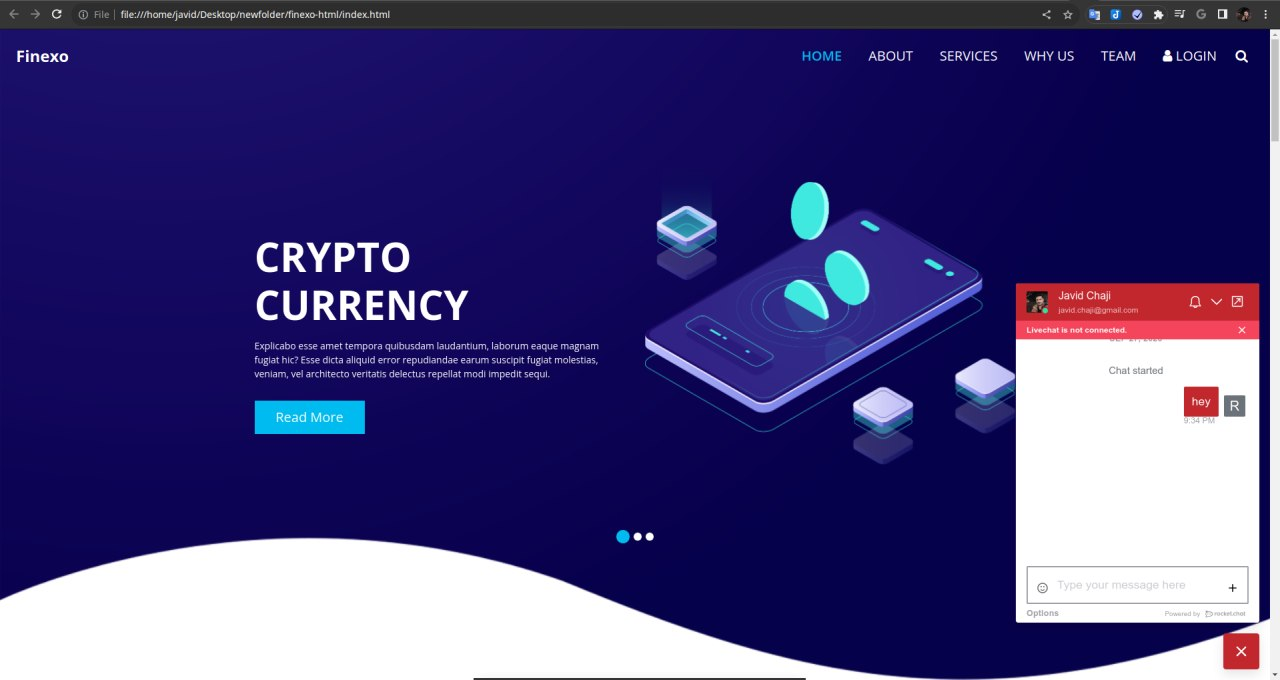
\includegraphics[width=\linewidth]{Images/Working_Chat_Widget_Example.jpg}
    \caption{نمونه اجرا شده‌ای از \lr{Chat Widget} در یک صفحه HTML اجرا شده‌ به صورت محلی}
\end{figure}


\subsection{گزارش روز پنجشنبه ششم مهرماه ۱۴۰۲}

۱۴۰۲/۰۷/۰۶

امروز درباره استفاده مستقیم مدل های زبانی بزرگ توسط Rocket.Chat جستوجو انجام دادم که به نظر با API های راکت چت می‌توان از مستقیم LLM ها را روی این پلتفرم اجرا کرد اما مسئله اینجاست که اگر من این کار را مستقیم و بدون استفاده از Rasa انجام دهم از بعضی تنظیمات پیچیده و پیشرفته چت بات محروم میشوم به طور مثال \lr{intent classification} یکی از آن هاست
امروز بیشتر سعی کردم تا ظاهر Rocket.Chat را به صورت شخصی سازی شده برای دانشگاه فردوسی دربیاورم عکس ها و نماد ها را عوض کردم ولی نتیجه ای نگرفتم احتمالا یا مشکل از کش کردن نماد هاست و یا نماد های اشتباهی را عوض کردم که احتمالش کم هست دلیل اینکه کمی تست ظاهر کمی کند تر جلو میرود این هست که اجرای راکت چت حدودا به ده دقیقه build نیاز دارد
دلیل انتخاب اسم سیمرغ برای این پروژه این هست که سیمرغ نماد راهنمایی، خرد و دانایی در شاهنامه فردوسی هست و ما در دانشگاه فردوسی هستیم و میخواهیم از راهنمایی این راهنما .استفاده کنیم


\subsection{گزارش روز جمعه هفتم مهرماه ۱۴۰۲}

۱۴۰۲/۰۷/۰۷

.امروز تغییر بعضی از آیکون ها و لوگو ها انجام شد و به دنبال بک گراند های مرتبط با دانشگاه گشتم (سعی کردم لوگو مناسبی برای چت بات انتخاب کنم ولی اگر نیاز باشد می‌شود که لوگوی مناسب تری هم درست کرد لوگوی فعلی سیمرغ نشانی هست که به عنوان نشان سلطنتی امپراتوری ساسانی به کار برده میشده) احتمالاً بک گراند با کیفیتی برای صفحه لاگین که نمایی از دانشگاه را داشته باشد پیدا کنم هنوز به مورد خوبی دست پیدا نکردم ولی سعی میکنم اول به معنای کار که چت بات هست برسم در همین حین احتمالاً با توجه به پرس و جو هایی که انجام دادم شاید کسی عکس باکیفتی از نمای سبز دانشگاه داشته باشه که در طول ساخت بقیه اعضای چت بات به دستم خواهد رسید.

در روز های آینده باید بیشتر با ساختار کد راکت چت آشنا بشم و تصمیم اینکه آیا از Rasa استفاده بشود یا نه را بگیرم ولی به احتمال زیاد از Rasa استفاده خواهم کرد.


\begin{figure}[h]
    \centering
    
\includegraphics[width=0.5\linewidth]{Images/Simurgh_Logo.png}
    \caption{لوگوی فعلی سیمرغ، نشانی که به عنوان نشان سلطنتی امپراتوری ساسانی به کار برده می‌شده است.}
\end{figure}


\subsection{گزارش روز شنبه هشتم مهرماه ۱۴۰۲}

۱۴۰۲/۰۷/۰۸

امروز به دنبال ساختار Rasa و تفاوت های NLU و LLM و chatbot های کمی قدیمی تر بودم. یک مدل تقریباً مناسب که Rasa را هم در خود داشت RasaGPT بود که خود Rasa را اجرا میکرد و با ChatGPT ترکیب میکرد و به صورت یک ربات تلگرام اجرا میشد و قابلیت پاسخگویی بدی نداشت اما این مدل کمی ضعیف بود و مشخص بود به اندازه \lr{Llama 2} خوب کار نمی‌کند. (البته بستگی به پارامتر ها و بیت سایز و دیتاست و ... هم دارد.)

بزرگترین مشکل پیش‌رو گردآوری داده کافی برای fine-tuning مدل هست که مهم ترین قدم نیز هست 
از این به بعد چون مشکلات UI بسیار کاهش پیدا کرده مقدار جزئیات باقی مونده از آن را برای بعد از بهبود دادن هوش خود چت بات می گذارم تا هر دو به موازات پیش بروند.


\subsection{گزارش روز یکشنبه نهم مهرماه ۱۴۰۲}

۱۴۰۲/۰۷/۰۹

امروز درباره SVG فایل ها کمی یاد گرفتم و برای حالت تاریک Rocket.Chat لوگوی SVG برنامه را عوض کردم تا در حالت تاریک contrast بهتری داشته باشد.
به طور کلی Rasa از سه قسمت یا مدل اصلی تشکیل شده است:

\begin{itemize}
    \item \lr{Rasa Core} : این قسمت یا مدل، مدیریت گفتوگوی چت بات را به عهده دارد که این کار را با کمک NLU انجام می‌دهد.
    \item \lr{Rasa NLU} : این قسمت یا مدل، اطلاعات مهم پیام کاربر را استخراج می‌کند مانند منظور\footnote{Intent} کاربر و ...
    \item \lr{Rasa T5} : این قسمت یا مدل، یک LLM هست که برای کارهایی از قبیل ترجمه و جمله سازی و پاسخ به پرسش ها استفاده می‌شود که نقش مهمی در کیفیت خروجی چت بات دارد به طور مثال اگر از \lr{Llama 2} به جای T5 استفاده کنیم.
\end{itemize}


\subsection{گزارش روز دوشنبه دهم مهرماه ۱۴۰۲}

۱۴۰۲/۰۷/۱۰

امروز درباره ساختار فایلی Rasa ویدئو های یوتیوب رسمی Rasa را مشاهده کردم.
این ویدئو ها درباره ساختار فایل ها در Rasa و نقش آنها در ساخت چت بات بود و یک ویدئو مخصوص فایل Domain بود که از مهم ترین فایل های Rasa هست در این فایل انواع Intent ها (که یک نوع دسته بندی پاسخ های کاربر هست) و همینطور Entites (که کلمات کلیدی استخراج شده از پرسش کاربر هست) و Slots (که یک نوع حافظه برای چت بات ما هست که نیاز داریم آن مورد را در طول مکالمه به خاطر داشته باشه) و پاسخ ها (که پاسخ هایی هست که در صورت اقدام به یک intent خاص باید به کاربر داده شود) قابل تعریف هستن که باعث می‌شوند Rasa هم به شکل قدیمی به صورت یک چت بات \lr{rule based} عمل کند و هم با استفاده از NLP و \lr{Machine Learning}؛ که برای کارهایی که از پیش تعریف شده است برای سرعت و راحتی از قسمت \lr{rule based} استفاده می کند و برای سناریو هایی که برای آن تعریف نشده از NLP و موارد دیگر استفاده می کند(البته در صورت نیاز به پاسخ دادن در مواردی که سناریو ای برای آن‌ها وجود ندارد، که آن هم قابل تعیین هست)


\subsection{گزارش روز سه‌شنبه یازدهم مهرماه ۱۴۰۲}

۱۴۰۲/۰۷/۱۱

امروز به دیدن ویدئو های مربوط به Rasa ادامه دادم، Rasa این ویژگی ها را دارد که در گفتوگو برای کاربر عکس ارسال کند و یا حتی دکمه هایی برای پاسخ های خاص دستیار تعیین شود تا در صورت نیاز به کاربر نمایش داده شود و کاربر بنابر خواسته یکی را انتخاب کند، همچنین می‌توان تنظیماتی قرار داد که اگر ارتباط کاربر با چت بات از طریق مثلاً slack بود پاسخی متفاوت با پاسخ معمولی که در همان شرایط به کاربری که از slack استفاده نمی کند بدهد.


\subsection{گزارش روز چهارشنبه دوازدهم مهرماه ۱۴۰۲}

۱۴۰۲/۰۷/۱۲

امروز ویدئو های آموزش داده ها و قوانین را دیدم. از نکات توصیه شده داشتن intent های کمتر هست چون از جهات زیادی باعث مشکل می‌شود به طور مثال با تعریف intent زیاد باعث می شویم که تعداد کلاس ها در زمان آموزش مدل زیاد شود و مدل طولانی تر آموزش ببیند همچنین با داشتن intent زیاد نیاز به داده زیاد نیز هست بنابراین کار سخت تر میشود کوتاه نگه داشتن سناریو های گفتگو از دیگر موارد مهم هست زیرا بتوان از این سناریوها برای ساخت سناریو های دیگر استفاده کرد اما به صورت کلی چون ما احتمالاً از مدل های زبانی بزرگ استفاده خواهیم کرد لازم نیست خیلی ذهن خودمان را درگیر این سناریوها کنیم فقط تا جایی که به خاطر می آوریم و در ادامه با چت کاربران با چت بات توانایی تشخیص سناریو های جدید را خواهیم داشت (طبق تاکید آموزگار این ویدئو هیچ وقت نمی توان همه سناریو های ممکن را در نظر گرفت)


\subsection{گزارش روز پنجشنبه سیزدهم مهرماه ۱۴۰۲}

۱۴۰۲/۰۷/۱۳

امروز به ویدئوی مربوط به Entity ها در Rasa را دیدم Entity ها در Rasa همان کلمات کلیدی ای هستند که از پاسخ کاربر استخراج می‌شوند
به طور مثال اگر کاربر بخواهد بلیط هواپیما از طریق ربات ما بگیرد مشخصات مبدأ و مقصد را باید از کلمات کاربر استخراج کنیم این کار در Rasa به سه روش انجام می‌شود. یک به صورت مدل های از پیش تعیین شده مثل مدل های قوی ای که در پایتون وجود دارد دوم با استفاده از \lr{Regular Expertion} و سوم با استفاده از ماشین لرنینگ، یکی دیگر از امکانات Entity ها توانایی استفاده از Synonym ها در Rasa هست که به ما این امکان را میدهد که اگر بخواهیم به طور مثال از متن کاربر برداشتی را داشته باشیم که با شکل های مختلف قابل بیان هست می‌توانیم همه را به یک بردار واحد مپ کنیم که همه را در نهایت جزو آن دسته قرار بدهیم
و این که می‌توانیم از Entity ها حتی در سناریو ها هم استفاده کنیم.


\subsection{گزارش روز جمعه چهاردهم مهرماه ۱۴۰۲}

۱۴۰۲/۰۷/۱۴

امروز به دیدن ویدئو های قسمت Slot ها در Rasa پرداختم که برای ذخیره جریان مکالمه و یا اطلاعات ضروری استفاده میشود و در فایل Domain تعریف می‌شوند و می‌توان با این ویژگی و Action و Entity که باید هم نام با Slot باشد یک مدل زبانی بزرگ و یا حتی یک منبع اطلاعات مانند دیتابیس را به Rasa متصل کرد و از آن استفاده برد.


\subsection{گزارش روز شنبه پانزدهم مهرماه ۱۴۰۲}

۱۴۰۲/۰۷/۱۵

امروز به دیدن ادامه ویدئو های قسمت Slot ها پرداختم، Slot ها در Rasa می‌توانند انواع مختلف باشند مانند \lr{Text, Boolean, Float, Category, Any} که هر کدام کاربرد خاص خود را دارند به طور مثال در Text می‌توان فلگی را فعال کرد که به چت بات بگوید این اطلاعاتی را که در این \lr{Text Slot} ذخیره کردی را در پاسخ بعدی خود به کاربر دخالت بده و به طور مثال اگر کاربر یکی از اطلاعات را کم وارد کرده باشد مجدداً از او می‌پرسد.


\subsection{گزارش روز یکشنبه شانزدهم مهرماه ۱۴۰۲}

۱۴۰۲/۰۷/۱۶

امروز ویدئو های مربوط به Respose ها در Rasa را دیدم پاسخ ها برای یک حالت خاص مثل خوش‌آمد می‌توانند چند پاسخ مجزا باشند که به صورت رندم چت بات یکی را انتخاب کند و همینطور می‌توان در پاسخ ها از دکمه کمک گرفت که کاربر با دکمه ها به ما پاسخ دهد و همچنین می‌توان در جملات پاسخ ها از متغیر استفاده کرد که همان‌طور که از قبل داشتیم با مقداری که در یک اسلات ذخیره کردیم می‌توانیم به کاربر پاسخی بدهیم که در آن از اطلاعات مخصوص به کاربر استفاده شده باشد.


\subsection{گزارش روز دوشنبه هفدهم مهرماه ۱۴۰۲}

۱۴۰۲/۰۷/۱۷

امروز ویدئوی مربوط به Pipeline و \lr{Policy Configuration} دیده شد که چطور انتخاب کردن رفتار ما با پیام کاربر از دیدگاه ماشین لرنینگ و \lr{Rule Based}  چت تعیین می‌شد به طور مثال اینکه چطور تعداد epoch ها را برای آموزش بهتر عوض کنیم و یا تعداد لایه ها را تغییر دهیم و اینکه بعد از گرفتن پیام کاربر به ترتیب چه کارهایی روی آن انجام دهیم که در مرحله آخر که Classification اینتنت ها قرار می‌گیرد. قوی ترین Classifier موجود برای دسته‌بندی Intent ها DIET نام دارد که ساخت سازندگان خود Rasa نیز هست.

به طور کلی Rasa :

\begin{enumerate}
    \item ابتدا \lr{Rules Policy} را نگاه میکند اگر می‌توانست با قوانین فایل به کاربر پاسخ دهد، پاسخ می‌دهد.
    \item در غیر این صورت به \lr{Memoization Policy} مراجعه می‌کند از فایل story.yml سناریوهای کلی ای که از قبل برای مکالمه با کاربر تعیین کردیم را استفاده می‌کند که کدام یک از این سناریو ها بهترین همخوانی را با گفتوگوی فعلی دارد.
    \item اگر این روش هم پاسخی در برنداشت از TED استفاده می‌کند که مخفف \lr{Transformer Embedded Dialogue} است و کار Generalize کردن دانسته های چت بات را انجام می‌دهد و پاسخ را با توجه به دانسته های کل چت بات به کاربر ارائه می‌دهد.
\end{enumerate}

ولی اگر هر سه، پاسخی برای کاربر داشتند پاسخ شماره ۱ به ۲ و ۲ به ۳ ارجحیت دارد.


\subsection{گزارش روز سه‌شنبه هجدهم مهرماه ۱۴۰۲}

۱۴۰۲/۰۷/۱۸

امروز به دیدن ویدئوی مربوط به \lr{Custom Actions} در Rasa پرداختم این ویژگی به ما کمک می‌کند توابع خودمان را به چت بات اضافه کنیم نکته و کاربرد اصلی این ویژگی توانایی دادن به چت بات برای ارتباط با دیتابیس و Api های مختلف هست که توانایی های آن را بالا میبرد به طور مثال ساعت را برای منطقه زمانی کاربر از Api سایت ساعت جهانی دریافت می‌کند.


\subsection{گزارش روز چهارشنبه نوزدهم مهرماه ۱۴۰۲}

۱۴۰۲/۰۷/۱۹

امروز ادامه \lr{Rasa Custom Actions} را مشاهده کردم، از نظر من برای ساخت چت بات \lr{Custom Actions} در Rasa بسیار کاربردی هست چون خیلی کار های جالبی می‌شود با آن انجام داد و تقریباً هر تسکی را قابل تعریف می‌کند. در ادامه این ویدئو شیوه پیاده سازی کلاس برای \lr{Custom Actions} گفته شد به طور مثال ما در هر کلاس یک متد run داریم که این متد یک Dispatcher و یک Tracker و یک Domain را به عنوان ورودی می‌گیرد این متغیرها اطلاعات لازم از چت و چت بات را به \lr{Custom Action} می‌دهند

مثلاً Dispatcher چت های قبلی کاربر را در اختیار ما می‌گذارد و Tracker وضعیت فعلی کاربر را مثلاً الان خوشحال هست و یا ناراحت و به صورت کلی Intent کاربر را و Domain هم برای استفاده از مواردی هست که در فایل domain.yml تعریف شده هست مثل Slot ها



\subsection{گزارش روز پنجشنبه بیستم مهرماه ۱۴۰۲}

۱۴۰۲/۰۷/۲۰

امروز ویدئوی مربوط به فرم ها در Rasa را مشاهده کردم با استفاده از فرم ها می توان از کاربر اطلاعات لازم را برای مثال برای سفارش پیتزا دریافت کرد ولی این فرم ها چگونه کار می‌کنند؟! فرم ها در Rasa از چند Slot تشکیل شده اند که به طور مثال برای سفارش پیتزا یک اسلات برای سایز پیتزا و یکی برای نوع پیتزا می‌توان قرار داد حال که کاربر درخواست سفارش پیتزا می‌کند این فرم سفارش پیتزا به حالت فعال در می آید اگر در درخواستش این اسلات ها را ذکر نکرده باشد چت بات به صورت خودکار از آن درخواست می‌کند لطفاً نوع پیتزا را انتخاب کنید که البته این نکته هم قابل ذکر است که ممکن است کاربر نوع پیتزایی را انتخاب کند که وجود ندارد و یا در منوی ما نیست در این صورت هم این قابلیت وجود دارد که همراه با \lr{Custom Actions} که در نهایت قرار است پیتزا را سفارش دهد طوری فرم را تنظیم کنیم که اگر کاربر پاسخ معتبری برای پر کردن اسلات های فرم نداد فرم مجدداً از کاربر سوال کند و در نهایت وقتی که تمام اسلات های فرم پر شدند، فرم به حالت غیر فعال در آمده و این یعنی شروع می‌کند به اجرای \lr{Custom Action}  ای که برایش تعریف شده است.


\subsection{گزارش روز جمعه بیست و یکم مهرماه ۱۴۰۲}

۱۴۰۲/۰۷/۲۱

امروز ویدئوی Form ها تمام شد موضوع امروز بیشتر پیاده سازی و نحوه ساخت \lr{Custom Action} برای فرم بود که به ازای هر Slot می‌توانیم یک تابع پیاده سازی کنیم که این تابع درون این نوع کلاس که از کلاس Validation ارث بری می‌کند می‌تواند در بررسی معتبر بودن ورودی کاربر به ازای مقادیر فرم به ما کمک کند.


\subsection{گزارش روز شنبه بیست و دوم مهرماه ۱۴۰۲}

۱۴۰۲/۰۷/۲۲

امروز ویدئوی مربوط به \lr{Custom Forms} را مشاهده کردم که درباره اینکه چطور می‌توان بیش از پیش فرم ها را در Rasa شخصی سازی کرد توضیح داده شد. به طور مثال ممکن است بعد از اینکه کاربر پیتزا سفارش می‌دهد بلافاصله بعد از ایجاد فرم و در زمانی که ربات از او می‌پرسد که چه نوع پیتزایی می‌خواهید کاربر به یک بحث متفرقه بپردازد در اینجا می‌توان با استفاده از Rule ها و اضافه کردن Rule مناسب پاسخ را مدیریت کرد ولی اگر کاربر خواست سفارش خود را لغو کند چطور؟ این مورد را باید در Story ها بیاوریم و با توجه به اینکه خود الگوریتم های \lr{Machine Learning} ای که در Rasa استفاده می‌شود کار Generalization برای Story ها را انجام می‌دهد از جهت اینکه کاربر چطور سفارش خود را لغو خواهد کرد کمی نگرانی کمتری خواهیم داشت و البته قطعاً Intent ای هم برای لغو سفارش قرار داده ایم.


\subsection{گزارش روز یکشنبه بیست و سوم مهرماه ۱۴۰۲}

۱۴۰۲/۰۷/۲۳

امروز ویدئوی مربوط به \lr{Custom Forms} تمام شد به نظرم در نهایت خیلی چیز تازه ای بیان نشد و کمی بیشتر به جزئیات کد پرداخت و اینکه مثلاً به مسیری که ما در چت بات پیشبینی کردیم \lr{happy path} می‌گوییم و به مسیر هایی که کاربر ممکن است برود و ما پیشبینی نکرده‌ایم \lr{unhappy path} گفته می‌شود و گذاشتن دکمه برای انتخاب مورد نظر می‌تواند در فرم ها به ما کمک کند این دکمه ها در RasaX رندر می‌شوند ( RasaX : یکی از UI های مربوط به Rasa هست و در واقع \lr{User Interface} رسمی ساخته شده توسط Rasa است.)



\subsection{گزارش روز دوشنبه بیست و چهارم مهرماه ۱۴۰۲}

۱۴۰۲/۰۷/۲۴

امروز ویدئوی \lr{Integration with website} را دیدم که ساختار کلی Rasa و نحوه اتصال Rasa از طریق \lr{Rest Api} به سایت ها و پلتفرم های مختلف را توضیح داده شد به نظرم این ویدئو جذاب ترین ویدئوی Rasa تا اینجا بود و برخلاف ویدئوی قبلی بسیار پرکاربرد بود و اگر با اطلاعات نسبتاً کمی هم دیده شود همچنان می‌تواند خیلی کمک کننده باشد مخصوصاً برای من که در برنامه نویسی وب ضعیف تر هستم.

\begin{figure}[h]
    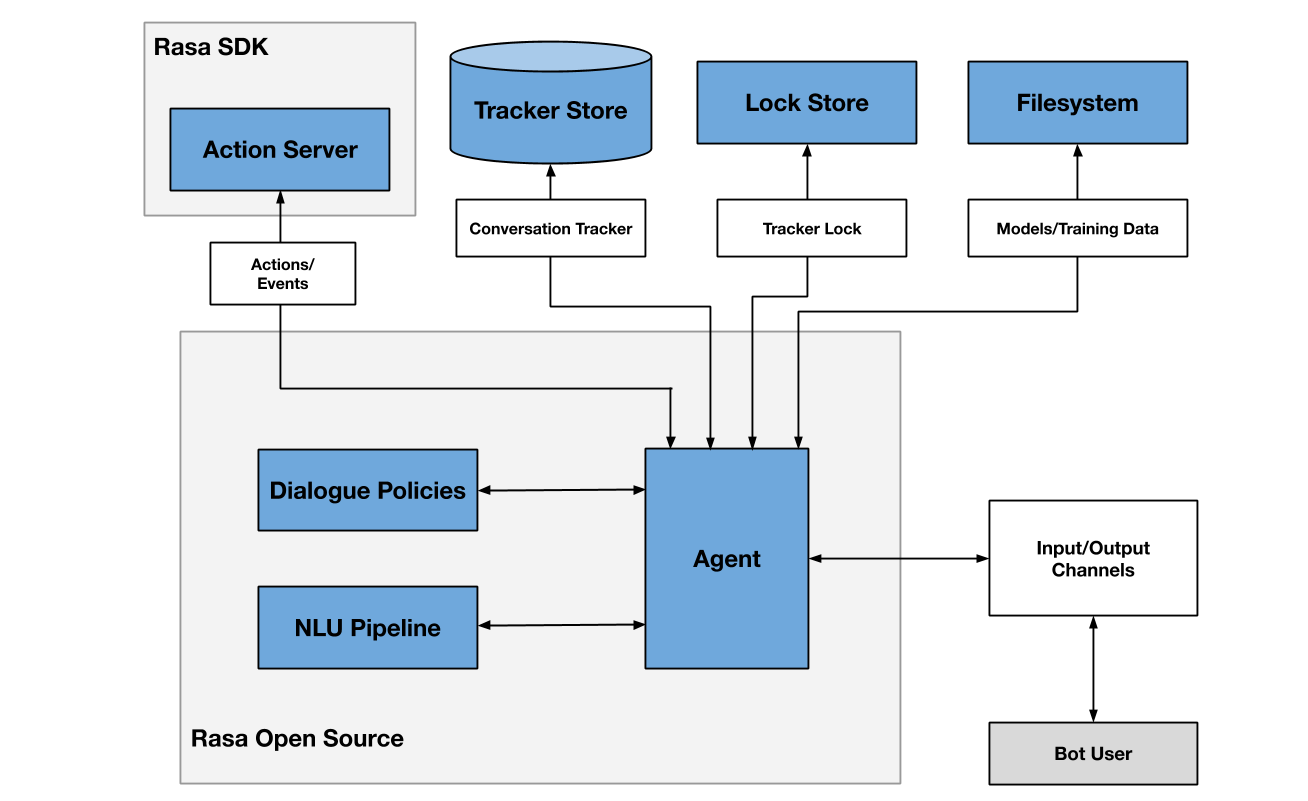
\includegraphics[width=\linewidth]{Images/Rasa_Architecture.png}
    \caption{معماری \lr{Rasa Open Source} طبق Documentation سایت این چهارچوب}
\end{figure}


\subsection{گزارش روز سه‌شنبه بیست و پنجم مهرماه ۱۴۰۲}

۱۴۰۲/۰۷/۲۵

امروز ویدئوی \lr{CDD \& RasaX} را مشاهده کردم که درباره توسعه ی مداوم Rasa و CI و CD آن بود که با RasaX که یک UI برای Rasa هست می‌توان این مقاصد را بسیار خوب برطرف کرد به طور مثال در RasaX به همه گفتوگوهای انجام شده دسترسی داریم و به راحتی قابلیت اصلاح و Retrain مدلمان را داریم و همینطور می‌توان با ساختن لینک Colleagues برای کسانی که می‌توانند با گفتوگو کردن با چت بات‌مان به بهتر شدن آن کمک کنند (توسط گفتوگو و ساخته شدن سناریو های ناشناخته که Intent از پیش تعریف شده ندارند) و دادن لینک به آنها به روش \lr{Conversation Driven Development} ربات را بهبود داد.


\subsection{گزارش روز چهارشنبه بیست و ششم مهرماه ۱۴۰۲}

۱۴۰۲/۰۷/۲۶

امروز ویدئوی RasaX به پایان رسید RasaX واقعاً کاربردی و مفید هست مخصوصاً اگر از Rasa اطلاعات خاصی نداشته باشیم می‌توانیم با اجرای Rasa و RasaX و آزمون و خطا تا حد خیلی خوبی متوجه شیوه کار Rasa شویم یکی از ویژگی های فوق‌العاده RasaX همگام شدن آن با GitHub هست که می‌توان همزمان با لیبل زدن پیام های دریافتی از کاربران آن ها را در گیت هاب کامیت کرد و بلعکس اگر تغییری روی گیت هاب بدهیم بعد از مدتی روی RasaX نیز این تغییر انجام می‌شود

از دوره \lr{NLP Specialization} امروز آزمون هفته اول را گذراندم بعد از ۴ مرتبه آزمون دادن ۱۰۰ از ۱۰۰ شد


\subsection{گزارش روز پنجشنبه بیست و هفتم مهرماه ۱۴۰۲}

۱۴۰۲/۰۷/۲۷

امروز ویدئوی مربوط به پیشرفت Rasa و چیز هایی که به تازگی به آن اضافه شده را دیدم و یک دسته بندی جالب داشت که عکسش بعد از گزارش ارسال می‌شود که درباره بلوغ \lr{Conversational AI} هست که البته به نظر من با توجه به توضیحات مدرس (تا جایی که متوجه شدم در زمان ضبط این سری ویدئو های آشنایی اولیه هنوز چت جی پی تی معرفی نشده بوده است) فکر میکنم الان در قسمت چهارم هستیم.

از دوره \lr{NLP Specialization} ویدئوی اول هفته دوم و همینطور ویدئوی مصاحبه با Chris Manning را دیدم

https://github.com/JavidChaji/DeepLearning.AI-Natural-Language-Processing-Specialization


\begin{figure}[h]
    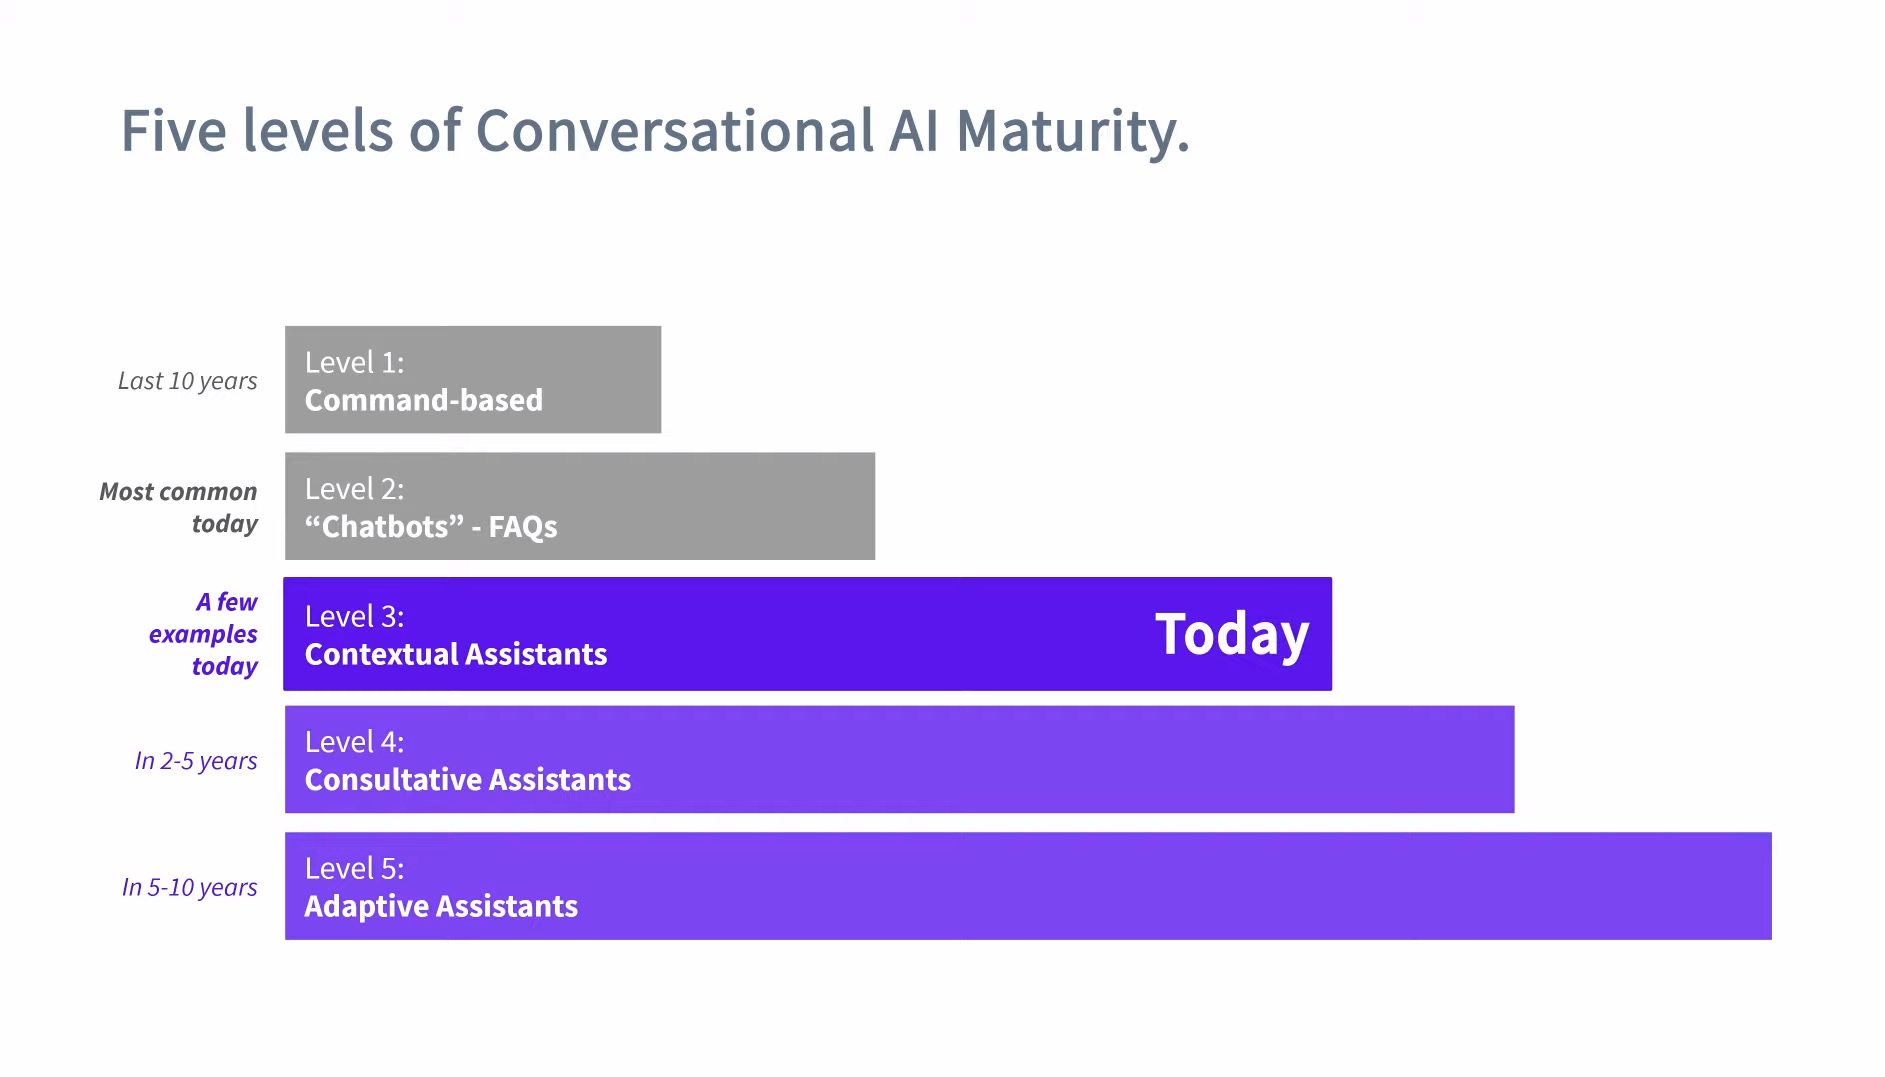
\includegraphics[width=\linewidth]{Images/Five_Level_of_Conversational_AI_Maturity.png}
    \caption{پنج سطح بلوغ \lr{Conversational AI}}
\end{figure}



\subsection{گزارش روز جمعه بیست و هشتم مهرماه ۱۴۰۲}

۱۴۰۲/۰۷/۲۸

امروز چند جلسه از \lr{NLP Specialization} را دیدم که قانون بیز و مقدمات آن را تدریس شد.

https://github.com/JavidChaji/DeepLearning.AI-Natural-Language-Processing-Specialization


\subsection{گزارش روز شنبه بیست و نهم مهرماه ۱۴۰۲}

۱۴۰۲/۰۷/۲۹

امروز به دنبال تاریخچه Rasa برای شروع اسلاید ها رفتم اینکه از ۲۰۱۶ توسط سه نفر ساخته شده و بعد ها ویژگی های جدیدی به آن اضافه شده و سازندگانش با الهام از Framework هایی مثل \lr{Tensor Flow} آن را ساخته‌اند به علت اینکه کمبود Framework ای در زمینه \lr{Conversational AI} احساس می‌شده است

امروز جلسات \lr{Naive Bayes} و \lr{Laplacian Smoothing} و  \lr{Log Likelihood} 
از دوره NLP Specialization را دیدم

https://github.com/JavidChaji/DeepLearning.AI-Natural-Language-Processing-Specialization


\subsection{گزارش روز یکشنبه سی‌ام مهرماه ۱۴۰۲}

۱۴۰۲/۰۷/۳۰

امروز یک پروژه جدید Rasa ساخته شد که با توجه به مراحل ساخت این پروژه، مراحل نصب و آماده سازی Rasa در فایل README.md ی پروژه قرار گرفت. این پروژه قرار است به همان چت بات مورد نظر ما تبدیل شود.


\subsection{گزارش روز دوشنبه یکم آبان‌ماه ۱۴۰۲}

۱۴۰۲/۰۸/۰۱

امروز به دنبال اتصال Rasa با Rocket.Chat بودم و به یک سری چالش های وب برخوردم که برای روز های آینده باید بیشتر روی آن کار کنم و البته با تست یک ویژگی برای اتصال این دو باعث شدم Rocket.Chat از دسترس خارج شود و مجدداً Rocket.Chat را حذف و Build کردم که درست شود. (اگر سرور ایمیل STMP و یا STMPs برای Rocket.Chat فعال نکردید دکمه Verified را برای Admin نزنید وگرنه در حالی که کلید از داخل روی دَر هست پشت دَر می‌مانید)
همچنین برای ارائه به دنبال ساختار مناسبی بودم که بتوان به بیان مطالب مهم و مرتبط بیشتر پرداخت از ChatGPT و Bard چند الگوی مختلف که کلیت بیان مطالب را شرح میداد گرفتم و تقریباً با اختلافات جزئی نزدیک به هم بودند.


\subsection{گزارش روز سه‌شنبه دوم آبان‌ماه ۱۴۰۲}

۱۴۰۲/۰۸/۰۲

امروز برای اسلایدها وقت گذاشتم و قسمت ها و زیر قسمت هایشان را تعیین کردم و در Beamer درباره \lr{Beamer Notes} که نت هایی هست که ارائه دهنده می‌تواند موقع ارائه در اسلاید ها برای از قلم نداختن چیزی قرار دهد
از دوره \lr{NLP Specialization} هم قسمت دوم \lr{Log Likelihood} را دیدم.

https://github.com/JavidChaji/DeepLearning.AI-Natural-Language-Processing-Specialization


\subsection{گزارش روز چهارشنبه سوم آبان‌ماه ۱۴۰۲}

۱۴۰۲/۰۸/۰۳

امروز اسامی جدول طبقه‌بندی سلسله مراتب تیتر های LaTeX را مجدداً پیدا کردم که برای اسلاید ها استفاده کنم.

از دوره \lr{NLP Specialization} هفته دوم یعنی \lr{Sentiment Analysis with Naïve Bayes} به پایان رسید.

https://github.com/JavidChaji/DeepLearning.AI-Natural-Language-Processing-Specialization


\subsection{گزارش روز پنجشنبه چهارم آبان‌ماه ۱۴۰۲}

۱۴۰۲/۰۸/۰۴

امروز ویدئوی استفاده Bert در Rasa را دیدم که بعضی از اشکالات و بعضی از خوبی های استفاده از این مدل و مدل های شبیه به این ذکر شد مثل arBert برای عربی و یا mBert که از حدود ۱۰۴ زبان پشتیبانی می‌کند.


\subsection{گزارش روز جمعه پنجم آبان‌ماه ۱۴۰۲}

۱۴۰۲/۰۸/۰۵

امروز ترتیب سرفصل های اسلاید ها و به صورت تقریبی زیر فصل های آن مشخص شد به نظرم اگر به خوبی برای درست شدن این اسلاید ها وقت بگذارم هم خودم بهتر خواهم فهمید درباره \lr{Conversational AI} و Rasa و همچنین باعث پیاده سازی بهتر پروژه و در نهایت ارائه بهتر در جلسه چت بات ها خواهد شد برای همین حداقل یک هفته برای کامل کردن اسلاید ها (از جمله تشکلیل \lr{Mind Map} برای \lr{Conversational AI} و \lr{Rasa}) وقت خواهم گذاشت.


\subsection{گزارش روز شنبه ششم آبان‌ماه ۱۴۰۲}

۱۴۰۲/۰۸/۰۶

امروز به دنبال رفع بعضی ارور های اسلاید ها بودم که متوجه شدم در Beamer اصلاً Chapter نداریم و فقط Part و Section و Subsection و Subsubsection داریم و حتی Paragraph و Subparagraph هم نداریم و اگر در داکیومنت ذکر شود \lr{Syntax Error} خواهیم داشت و اینکه Documentation خودِ Beamer خوانا و خوب نوشته شده و خیلی کاربردی تر از چت بات ها هست برای پیداکردن پاسخ بعضی سوالات (همین الان که این متن را می‌نوشتم یک ایده به ذهنم رسید اینکه آیا ممکن هست بشود به جای Documentation هر پلتفرمی یک چت بات برایش ساخت تا به جای جستوجو در Documentation از Chatbot چیزی که میخواهیم را بپرسیم (البته این مورد را باید در نظر داشت که دیگر هر جمله از Documentation برای چت بات ما حکم یک حقیقت \footnote{Fact} خواهد داشت.) به طور مثال یک مدل زبانی پایه داشته باشیم که به صورت خیلی خوبی همه زبان ها را آموزش دیده باشه و بعد به ازای هر Documentation ای که میخواهیم چت باتش را بسازیم آن را fine-tune کنیم در نهایت شاید بشود این fine-tuning ها را Portable کرد تا شاید مثل pdf های الان که با \lr{PDF Reader} ها باز میشوند با یک برنامه که مدل پایه زبانی را دارد آن ها را باز کنیم تا بتوانیم سوالاتمان را از این چت بات که برای این Documentation فاین تیون شده بپرسیم)

از دوره \lr{NLP Specialization} آزمون هفته دوم را بعد از اولین مرتبه دادن ۷۰ شدم (نمره قبولی ۸۰ به بالا هست)


\subsection{گزارش روز یکشنبه هفتم آبان‌ماه ۱۴۰۲}

۱۴۰۲/۰۸/۰۷

امروز یک مدل دیگر چت بات برای بنده ارسال شد که طبق استاندارد های ارسال کننده به نظر بهتر از Rasa هست من از ایشون درباره دلایل برتری این مدل دیگر پرسیدم و منتظر هستم ببینم پاسخشون چه خواهد بود فردا باید یک نگاهی به این مدل کنم و با Rasa آن را مقایسه کنم (هنوز درباره Community این مدل اطلاعی ندارم ولی میدونم که \lr{Rasa Community} قابل قبول و شلوغی دارد و این خودش نکته مثبتی برای آینده دار بودن چهارچوب هست که در آینده نیاز به تعویض مدل به دلیل قدیمی شدن آن نداشته باشیم.)

از دوره \lr{NLP Specialization} برای مرتبه دوم و سوم آزمون هفته دوم را دادم و در مرتبه دوم ۹۰ و مرتبه سوم ۱۰۰ شدم و جلسه اول هفته سوم را شروع کردم.

https://github.com/JavidChaji/DeepLearning.AI-Natural-Language-Processing-Specialization


\subsection{گزارش روز دوشنبه هشتم آبان‌ماه ۱۴۰۲}

۱۴۰۲/۰۸/۰۸

امروز به مطالعه روش پیشنهادی پرداختم به نام Langchain ولی به نظرم تا جایی که دیدم هیچ برتری ای به \lr{Rasa Open Source}  نداشت در بهترین حالت با Rasa برابر بود ولی به هر حال منتظر خواهم شد جناب مهندس دلایلشون را بیان کنن و این سوال خیلی مهم برای من پیش آمده که اگر بخواهیم داده های خاص خودمان را روی Rasa فاین تیون کنیم در حالی که روی LLM مان تغییری ایجاد نکنیم (به این معنا که به صورت خام به Rasa داده شود و به صورت fine-tune شده در اختیار Rasa قرار نگیرد) آیا Rasa این قابلیت را دارد که این داده های ما را بدون اضافه کردنشان به example ها در فایل های domain.yml به صورت دیگری طوری یاد بگیرد به صورتی که خروجی چت بات با fine-tuning این داده ها به صورت مستقیم روی LLM مان تفاوتی نکند!



\subsection{گزارش روز سه‌شنبه نهم آبان‌ماه ۱۴۰۲}

۱۴۰۲/۰۸/۰۹

امروز درباره Example ها در Rasa بیشتر تحقیق کردم به نظر که راهی وجود دارد که لزوماً از Example ها استفاده نکنیم و همینطور امروز قسمتی از اسلاید ها را بهبود دادم.

از دوره \lr{NLP Specialization} چند قسمت از \lr{Vector Spaces} و \lr{word by word / word by document} را دیدم.

https://github.com/JavidChaji/DeepLearning.AI-Natural-Language-Processing-Specialization


\subsection{گزارش روز چهارشنبه دهم آبان‌ماه ۱۴۰۲}

۱۴۰۲/۰۸/۱۰

امروز از Documentation مربوط به Beamer چند نکته که جالب بود خواندم که بسیار کمک کننده بود به طور مثال با اینکه استفاده از Subsubsection در Beamer مجاز هست ولی به شدت نهی شده بود (چون ذهن مخاطب را نسبت به اسلاید مشوش می‌کند) و یا اینکه اگر ارائه ای طولانی باشه به طور مثال ۹۰ دقیقه می‌توان از Part استفاده کرد که هر پارت \lr{Table of Contents} خودش را دارد و نکته دیگر این بود که Section های هر پارت بیش از ۴ عدد نشود چون برای مخاطب بین ۲ تا ۴ Section قابل یادآوری هست ولی بیش از آن به خاطر سپاری آن سخت است. 
همچنین امروز مجدداً روی وصل کردن Rasa به Rocket.Chat کار کردم اتصال برقرار شده ولی اروری در رابطه با Webhook دریافت می‌کنم که باید برطرفش کنم تا ارتباط کامل برقرار شود. (هنوز متنی رد و بدل نمی‌شود.)



\subsection{گزارش روز پنجشنبه یازدهم آبان‌ماه ۱۴۰۲}

۱۴۰۲/۰۸/۱۱

امروز مجدداً برای اتصال Rasa و Rocket.Chat اقدام کردم و در نهایت توانستم یکی از پیام های Rasa را روی Rocket.Chat ببینم اما بعد از ۲۰ دقیقه این پیام آمد که یعنی هنوز مشکل اتصال داریم که باید بیشتر تست و جستجو برای حل مشکل اتصال انجام بدهم برای اتصال Rocket.Chat به Rasa هم Rasa و هم Rocket.Chat به کانفیگ های متناسب نیاز دارند به طور مثال این کانفیگ ها در Rasa در فایل credentials.yml قرار میگیرد و در Rocket.Chat باید یک user به عنوان بات تعریف کرد و یک \lr{Outgoing Webhook} برای آن User به همراه اطلاعات سرور Rasa تعریف کرد که البته Rocket.Chat یک برنامه\footnote{برنامه های Rocket.Chat چیزی شبیه افزونه ها برای مرورگر و یا Extension ها برای \lr{Visual Studio Code} هستند.} هم دارد به نام Rasa که از طریق API های Rasa با Rasa ارتباط برقرار می‌کند.

امروز از دوره NLP Specialization، فاصله اقلیدسی و cosine similarity را گذراندم.

https://github.com/JavidChaji/DeepLearning.AI-Natural-Language-Processing-Specialization


\subsection{گزارش روز جمعه دوازدهم آبان‌ماه ۱۴۰۲}

۱۴۰۲/۰۸/۱۲

امروز در ادامه تلاش برای اتصال Rasa به Rocket.Chat سعی کردم منبعی پیدا کنم تا دقیق تر نحوه اتصال را توضیح دهد در نهایت یکی از مخازن خودِ Rocket.Chat درباره این موضوع نوشته بود که با انجام مراحل آن و استفاده از Ngrok برای آشکار \footnote{Expose} کردن پورت Rasa برای دسترسی راحت ترِ Rocket.Chat به آن به این موضوع رسیدم که چیزی که Rasa در  دامنه Webhook خود برمی‌گرداند یک صفحه ساده HTML هست و باید از اینجا بیشتر راجع به کارکردن آن تحقیق کنم.


\subsection{گزارش روز شنبه سیزدهم آبان‌ماه ۱۴۰۲}

۱۴۰۲/۰۸/۱۳

امروز مشکل اتصال Rasa به Rocket.Chat حل شد ولی مشکلی که وجود داشت این بود که در پاسخ یک پیام Rasa چند پیام به مدت طولانی  پاسخ می‌داد که این مشکل هم برطرف شد و الان همانطور که عکس آن هم ضمیمه خواهد شد چت بات ما Rasa در Rocket.Chat تقریباً \footnote{چون هنوز یک اشکال کوچک هست که وقتی که Rasa می‌خواهد یک Session با Rocket.Chat را ببندد به طور مثال وقتی کاربری که سوالی پرسیده بعد از ۲۰ دقیقه پیامی ارسال نکند Rasa اقدام به بستن Session آن کاربر می‌کند که باعث می‌شود آخرین پیامی که Rasa به کاربر داده است مجدداً برای کاربر ارسال شود که البته هنوز این مشکل بررسی کامل نشده} به خوبی کار می‌کند و از مشکلات پیش رو، یکی پیدا کردن مدل زبانی فارسی مناسب هست (یا یک \lr{LLM}) و دیگری اضافه کردن قابلیت پشتیبانی زبان فارسی به Rasa (که با توجه به تحقیق های بنده ابزار هایی درست شده اند برای \lr{Rasa}) و نمایش درست آن در Rocket.Chat یا هر Frontend ای که مورد نظر باشد.


\begin{figure}[h]
    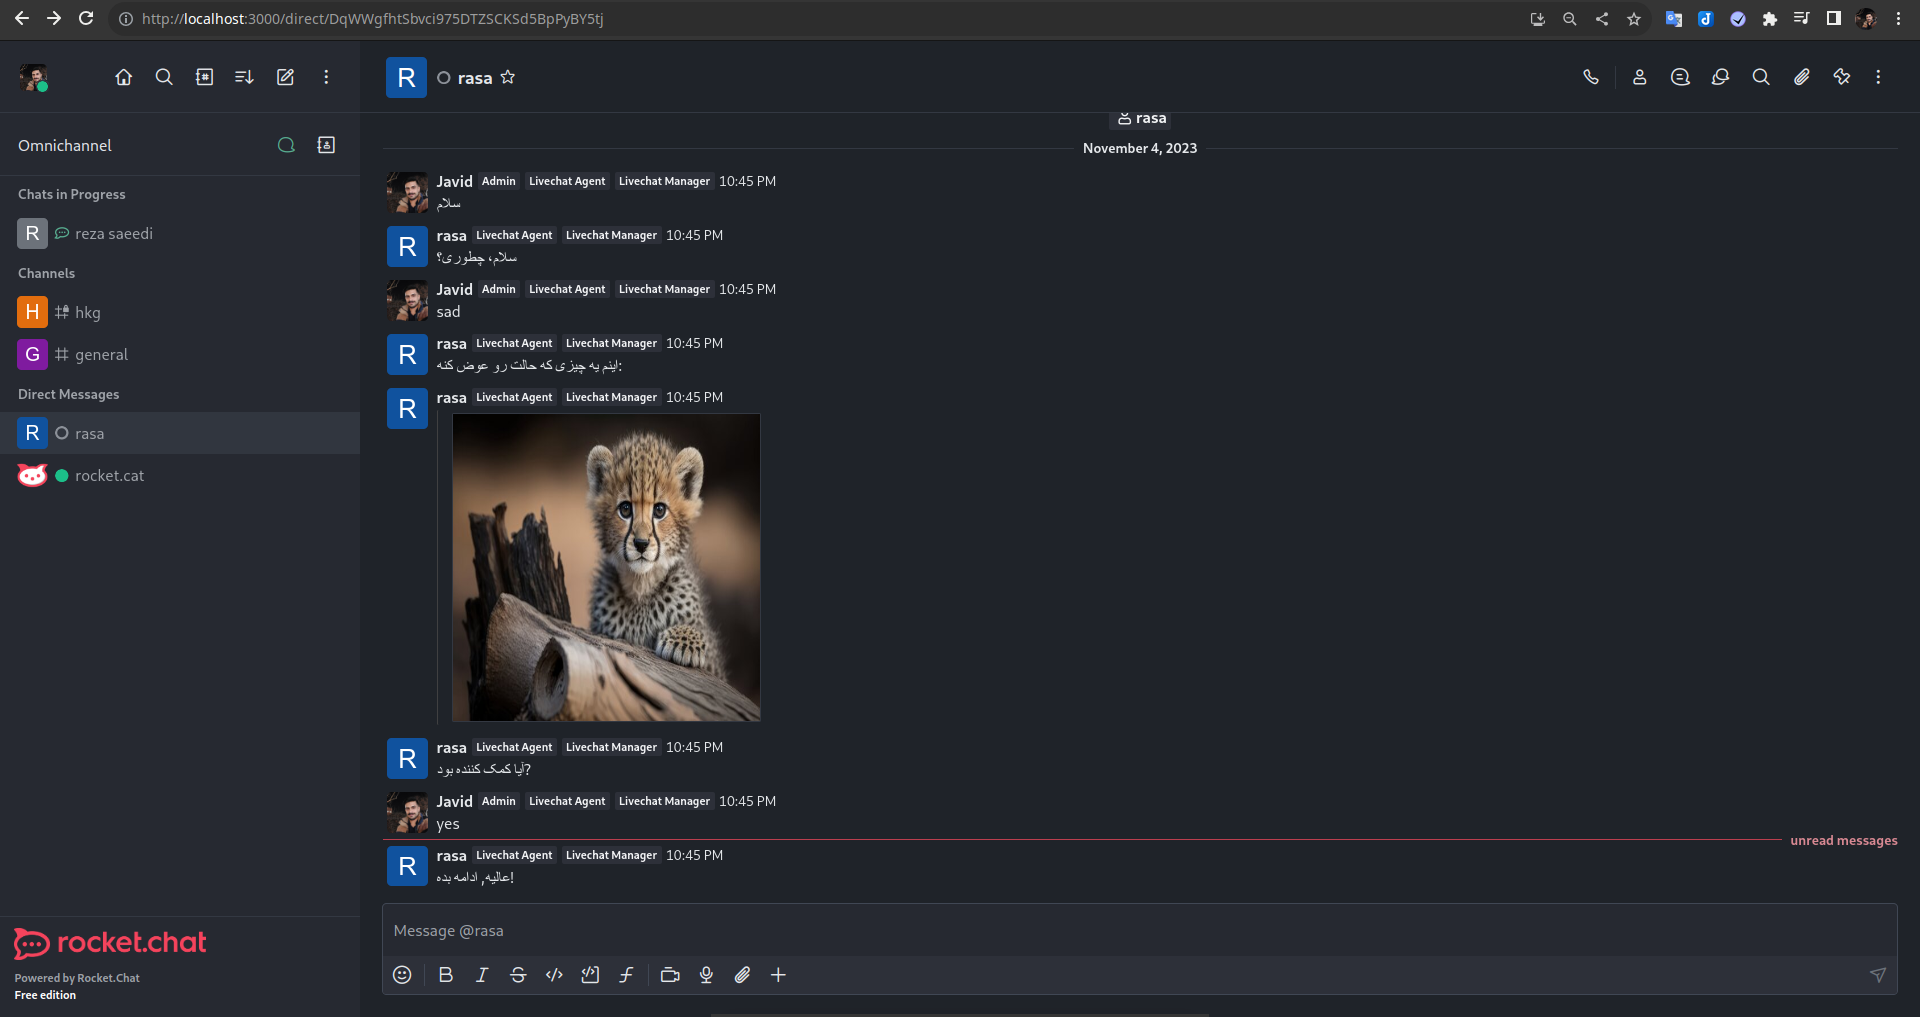
\includegraphics[width=\linewidth]{Images/Working_Connected_Rocket.Chat_Rasa_Example.png}
    \caption{نمونه متصل شده Rasa و Rocket.Chat و در حال گفتوگو}
\end{figure}



\subsection{گزارش روز یکشنبه چهاردهم آبان‌ماه ۱۴۰۲}

۱۴۰۲/۰۸/۱۴

امروز مراحل اتصال Rocket.Chat به Rasa را در فایل README.md ی مخزن پروژه اضافه کردم تا برای دفعات بعدی کار راحت باشد و همینطور کمی فایل README.md را مرتب کردم و لوگو و تصویر product (موقتی) به آن اضافه کردم.

از دوره \lr{NLP Specialization} قسمت \lr{Cosine Similarity} را گذراندم.

https://github.com/JavidChaji/DeepLearning.AI-Natural-Language-Processing-Specialization


\subsection{گزارش روز دوشنبه پانزدهم آبان‌ماه ۱۴۰۲}

۱۴۰۲/۰۸/۱۵

امروز هفته سوم دوره \lr{NLP Specialization} به پایان رسید موضوعات آن درباره PCA و \lr{Cosine Similarity} و \lr{Euclidean Distance} بود آزمون این هفته را هم با اولین مرتبه شرکت با نمره ۱۰۰ گذارندم و همینطور دو جلسه اول هفته چهارم را گذراندم



\subsection{گزارش روز سه‌شنبه شانزدهم آبان‌ماه ۱۴۰۲}

۱۴۰۲/۰۸/۱۶

امروز درباره دستور fine-tuning در Rasa کمی مطالعه کردم که اینطور که پیداست اگر یک فایل دیتا به هر شکلی به طور مثال CSV داشته باشیم می‌توانیم این داده ها را با دستور 
\begin{minted}[
framesep=2mm,
baselinestretch=1.2,
bgcolor=LightGray,
fontsize=\footnotesize,
linenos
]{bash}
  $ rasa train --finetune
\end{minted}
به عنوان داده هایی که برای fine-tuning در training استفاده می‌شود به آن داد و همینطور epoch های آن هم قابل ذکر هست به طور مثال به شکل \lr{-epoch-fraction 0.2} ولی برداشت بنده این هست که به طور کلی اگر بخواهیم چیزی را به صورت واقعیت به چت بات مان یاد بدهیم باید آن ها را در example های پاسخ و سناریو ها قرار دهیم.

امروز قسمت های مربوط به \lr{Transforming Word Vectors} که توسط \lr{Frobenius Norm} انجام می‌شد به نظرم خیلی جذابه که این تبدیلات با ریاضی میتونن معنای پشت کلمات را برامون شفاف کنن


\subsection{گزارش روز چهارشنبه هفدهم آبان‌ماه ۱۴۰۲}

۱۴۰۲/۰۸/۱۷

امروز اسلاید ها را برای ارائه کمی پیش بردم و همچنان به دنبال ساختار مناسب برای ارائه بودم. کار های مهم پیش‌رو برای پروژه زبان فارسی پروژه و انتخاب مدل هست که هر دو برای Rasa باید تعیین و تنظیم شوند.


\subsection{گزارش روز پنجشنبه هجدهم آبان‌ماه ۱۴۰۲}

۱۴۰۲/۰۸/۱۸

امروز قسمت های \lr{K-Nearest Neighbors} و \lr{Hash Table} و \lr{Hash Function} را از دوره \lr{NLP Specialization} دیدم که برای پیدا کردن نزدیک ترین معنای کلمه در زبان مورد ترجمه پس از حدس بردار کلمه آن در زبان مقصد کاربرد دارد که \lr{Hash Value} ها هر کدام شامل عناصری خواهند بود که نیاز هست از بین آن ها معنای کلمه مان را پیدا کنیم نه کلمات \lr{Hash Value} های دیگر.

https://github.com/JavidChaji/DeepLearning.AI-Natural-Language-Processing-Specialization


\subsection{گزارش روز جمعه نوزدهم آبان‌ماه ۱۴۰۲}

۱۴۰۲/۰۸/۱۹

امروز به جزئیات ظاهری اسلاید ها اعم از مواردی که در داکیومنت Beamer ذکر شده بود پرداختم ماننده اضافه کردن موسسه مرتبط و مواردی مانند اضافه کردن لیست فهرست در اسلاید ها که به شنوندگان کمک کند که الان در چه نقطه ای از ارائه هستیم (الخصوص در ارائه های ۹۰ دقیقه‌ای و نه ۱۰ دقیقه‌ای)

امروز قسمت های \lr{Locally Sensitive Hashing} و \lr{Multiple Planes} را از دوره \lr{NLP Specialization} گذراندم

https://github.com/JavidChaji/DeepLearning.AI-Natural-Language-Processing-Specialization


\subsection{گزارش روز شنبه بیستم آبان‌ماه ۱۴۰۲}

۱۴۰۲/۰۸/۲۰

امروز به گذراندن دوره \lr{NLP Specialization} مشغول بودم که به طور کلی درباره \lr{Approximate Nearest Neighbors} و \lr{Searching Documents} بود، هفته چهارم از دوره اول نیز به اتمام رسید و الان دو قسمت مقدمه دوره دوم از چهار دوره \lr{NLP Specialization} را شروع کرده ام

https://github.com/JavidChaji/DeepLearning.AI-Natural-Language-Processing-Specialization


\subsection{گزارش روز یکشنبه بیست و یکم آبان‌ماه ۱۴۰۲}

۱۴۰۲/۰۸/۲۱

امروز ویدئوی Rasa درباره مدلهای زبانی و ChatGPT دیدم و اینکه به طور مثال Bert و GPT هر دو یک مدل Transformer هستند با این تفاوت که Bert یک مدل Auto-Encoding هست و یعنی فقط روی قسمت \lr{Transformer Encoder} آموزش می‌بیند و دوطرفه هست ولی GPT یک مدل \lr{Auto Regressive} هست و فقط روی \lr{Transformer Decoder} آموزش می‌بیند و یک طرفه هست.


\subsection{گزارش روز دوشنبه بیست و دوم آبان‌ماه ۱۴۰۲}

۱۴۰۲/۰۸/۲۲

امروز به دنبال ویدئویی برای توضیح دقیق تر نحوه کار با LLM ها در Rasa بودم که خیلی نتیجه مفیدی نداشت مخصوصاً درباره زبان فارسی ولی باید به دنبال تغییر Pipeline باشم تا بتوانم در این قسمت مدل های زبانی فارسی را استفاده کنم.


\subsection{گزارش روز سه‌شنبه بیست و سوم آبان‌ماه ۱۴۰۲}

۱۴۰۲/۰۸/۲۳

امروز با جستوجو درباره Rasa و زبان فارسی کمی بیشتر درباره آن اطلاعات کسب کردم که به طور مثال Tokenizer و Featurizer هایی موجود هستن مانند FastText که یک Featurizer هست که بیش از 157 زبان دنیا را پشتیبانی می‌کند و دارای \lr{Vector Space} این زبان ها به صورت یکجا هست که البته اگر بخواهیم مستقیم از این مدل استفاده کنیم ۶ تا  ۷ گیگابایت حافظه اشغال می‌کند.

\subsection{گزارش روز چهارشنبه بیست و چهارم آبان‌ماه ۱۴۰۲}

۱۴۰۲/۰۸/۲۴

امروز به دنبال مطالب در Rasa برای ارائه بودم و تصمیم گرفتم ارائه طبق Documentation باشد تا هم جدید باشد و هم اگر نکته خاصی وجود داشت ذکر شود در حال درست کردن یک سلسه مراتب از ارائه هم هستم.

\subsection{گزارش روز پنجشنبه بیست و پنجم آبان‌ماه ۱۴۰۲}

۱۴۰۲/۰۸/۲۵

امروز درباره \lr{Conversational AI} جستوجو کردم که ببینم آیا مقاله ی Review ی مناسبی برای این موضوع وجود دارد که بشود با استناد به آن در ارائه چند اسلاید ابتدایی را راجع به تاریخچه ی \lr{Conversational AI} صحبت کنم که به نظر می‌آید که مقاله ی Review خیلی محکم و خوبی در این رابطه وجود ندارد ولی چند مقاله بودند که آن ها هم بیشتر روی یک سری جزئیات \lr{Conversational AI} مقاله Review داده بودند احتمالاً قسمت هایی از این دو سه مقاله ای که مرتبط تر بودند را برای تاریخچه \lr{Conversational AI} استفاده خواهم کرد (دلیل تاکید من روی گفتن تارخچه Rasa و همین‌طور \lr{Conversational AI} این هست که اگر خودم دانشجویی بودم که می‌خواستم در یک جلسه در مورد \lr{Conversational AI} چیزی بدانم خیلی لذت میبردم که ابتدا بدانم چی شده که ما رسیدیم به این نقطه و البته کمی باعث حس مسلط تر شدن به موضوع را هم به مخاطب منتقل می‌کند.)


\subsection{گزارش روز جمعه بیست و ششم آبان‌ماه ۱۴۰۲}

۱۴۰۲/۰۸/۲۶

امروز روی اسلاید ها کار کردم و تفاوت Rasa و \lr{Rasa Pro} را به اسلاید ها اضافه کردم همینطور تعریف \lr{Conversational AI} 
به نظر اگر از Documentation خود Rasa برای ترتیب ارائه مفاهیم استفاده کنم به مشکل بر خواهم خورد چون حس می‌کنم در نوشتن Documentation کمی خساست به خرج دادند و احتمال دارد به علت \lr{Rasa Enterprise} باشد ولی نیاز های اساسی و مفاهیم کلی را می‌توان از آن استخراج کرد.

از دوره NLP Specialization چند قسمت مربوط به auto correction را گذراندم.

https://github.com/JavidChaji/DeepLearning.AI-Natural-Language-Processing-Specialization


\subsection{گزارش روز شنبه بیست و هفتم آبان‌ماه ۱۴۰۲}

۱۴۰۲/۰۸/۲۷

امروز به تنظیم و گردآوری مطالب اسلاید ها به اسلاید ها پرداختم که بعد از اتمام این فرآیند باید مطالب گردآوری شده اصلاح و پالایش شوند برای اسلاید های نهایی در حال حاضر فقط مطالبی که قرار است گفته شود از Documentation خود Rasa استخراج می‌شود و اگر بعدا نیازی به توضیح بیشتر بود اضافه خواهد شد.

از دوره \lr{NLP Specialization} قسمت های ساخت مدل را گذراندم.

https://github.com/JavidChaji/DeepLearning.AI-Natural-Language-Processing-Specialization


\subsection{گزارش روز یکشنبه بیست و هشتم آبان‌ماه ۱۴۰۲}

۱۴۰۲/۰۸/۲۸

امروز در ادامه گردآوری مطالب اسلاید ها قسمت اول Concept ها به پایان رسید الآن که به دسته بندی مطالب Documentation خود Rasa نگاه میکنم دسته بندی بدی هم ندارد و اتفاقا خیلی خوب است ولی به هر حال باید در یک اسلاید دسته بندی شفاف تری ارائه بدم که قابل فهم تر شود.

از دوره \lr{NLP Specialization} قسمت \lr{Minimum edit distance} را گذراندم.

 https://github.com/JavidChaji/DeepLearning.AI-Natural-Language-Processing-Specialization


\subsection{گزارش روز دوشنبه بیست و نهم آبان‌ماه ۱۴۰۲}

۱۴۰۲/۰۸/۲۹

امروز در ادامه گردآوری مطالب اسلاید ها تا حدودی ساختار اسلاید ها را بر اساس ساختاری که در Documentation خود Rasa ارائه شده بود تغییر دادم و همینطور چند تا از ارور های LaTeX را برطرف کردم.

از دوره \lr{NLP Specialization} قسمت توضیح \lr{Minimum Edit Distance} با برنامه نویسی پویا را گذراندم.

https://github.com/JavidChaji/DeepLearning.AI-Natural-Language-Processing-Specialization


\subsection{گزارش روز سه‌شنبه سی ام آبان‌ماه ۱۴۰۲}

۱۴۰۲/۰۸/۳۰

امروز فقط کمی از ابتدای قسمت Concept های Rasa را مطالعه کردم.


\subsection{گزارش روز چهارشنبه یکم آذر‌ماه ۱۴۰۲}

۱۴۰۲/۰۹/۰۱

امروز هفته اول دوره \lr{NLP Specialization} به جز آزمون و نوت های هفته به پایان رسید در این هفته از \lr{Auto correct} و \lr{Edit Distance} و الگوریتم آن ها و برنامه نویسی پویا صحبت شد.

https://github.com/JavidChaji/DeepLearning.AI-Natural-Language-Processing-Specialization


\subsection{گزارش روز پنجشنبه دوم آذر‌ماه ۱۴۰۲}

۱۴۰۲/۰۹/۰۲

امروز خواندن نوت های هفته اول به پایان رسید و آزمون هفته اول گذرانده شد دفعه اول با نمره ۶۰ و دفعه دوم با نمره ۱۰۰.

https://github.com/JavidChaji/DeepLearning.AI-Natural-Language-Processing-Specialization


\subsection{گزارش روز جمعه سوم آذرماه ۱۴۰۲}

۱۴۰۲/۰۹/۰۳

امروز به دنبال درست کردن مانیتور برای کم بودن فضای Desktop بودم که با مشکل درایور های display  برخورد کردم که در نهایت با حذف درایور اینتل آن مشکل برطرف شد (چون هم Nvidia نصب بود و هم اینتل (آشپز که دو تا شد ... ))


\subsection{گزارش روز شنبه چهارم آذر‌ماه ۱۴۰۲}

۱۴۰۲/۰۹/۰۴

امروز با دو مانیتوره شدن خیلی راحت تر و سریع تر بخش های \lr{Training Data Formats} اسلاید ها ساخته شد در این بخش از ساخت اسلاید ها ابتدا ساختار اسلاید ها را شبیه به ساختار Documentation خود Rasa باز سازی کردم و به این نتیجه رسیدم که بهتره به جای داشتن یک ساختار قابل فهم و ساده که زمان زیادی می‌
برد که مفاهیم را برای چیدن درون این ساختار ساده منعطف کنیم به ساخت اسلایدها از ساختار کمی پیچیده تر خود Documentation استفاده کنم ولی این ساختار را با تیتر های قابل فهم و ساده بیشتر قابل هضم کنیم مخصوصاً با مثال های قابل لمس برای مخاطبین 
تا الان نوت های تقریبا یک سوم اسلاید ها آماده شده کم و بیش و بعد از کامل شدن نوت های اسلاید ها خود اسلاید ها و بعد هم ترجمه اسلاید را آماده خواهم کرد (ابتدا اسلاید ها را به زبان انگلیسی آماده میکنم که از نظر latex راحت تر هست و همینطور دقت تعاریف مفاهیم چون در خود زبان انگلیسی تعریف شده بیشتر خواهد بود.)

از دوره \lr{NLP Specialization} قسمت های ابتدایی هفته دوم را گذراندم که شامل مقدمات \lr{Part of Speech Tagging} می شد.

https://github.com/JavidChaji/DeepLearning.AI-Natural-Language-Processing-Specialization


\subsection{گزارش روز یکشنبه پنجم آذر‌ماه ۱۴۰۲}

۱۴۰۲/۰۹/۰۵

امروز در ادامه آماده سازی اسلاید ها یک قسمت و نیم دیگر تمام شد که شامل \lr{NLU Data Training} بود.

از دوره \lr{NLP Specialization} قسمت \lr{Makov Chain} را گذراندم.

https://github.com/JavidChaji/DeepLearning.AI-Natural-Language-Processing-Specialization


\subsection{گزارش روز دوشنبه ششم آذرماه ۱۴۰۲}

۱۴۰۲/۰۹/۰۶

امروز قسمت Domain هم به نوت های اسلاید ها اضافه شد و با نیم نگاهی که به قسمت های پیش رو داشتم به نظرم آمد که خیلی خیلی کوتاه باید از هر قسمت رد بشم چون واقعاً مطالب و جزئیات زیادی وجود دارد که که فرصت نخواهد شد دربارشون حرف زده شود.

از دوره \lr{NLP Specialization} قسمت \lr{Makov Chain and POS Tags}.

https://github.com/JavidChaji/DeepLearning.AI-Natural-Language-Processing-Specialization



\subsection{گزارش روز سه‌شنبه هفتم آذرماه ۱۴۰۲}

۱۴۰۲/۰۹/۰۷

برای تبدیل پایپلاین Rasa که فارسی را به آن بیفزاییم ابتدا باید یک \lr{Persian Tokenizer} داشته باشیم از بین \lr{Persian Tokenizer} های فارسی Hazm و Farasa و SpaCy که دقت SpaCy از دو تای دیگر کمتر است و برای استفاده همه منظوره hazm از دو تای دیگر بهتر هست و برای \lr{Named Entity Recognition (NER)}، Farasa بین این سه بی رقیب است
به نظرم برای پروژه hazm بهتر باشد با توجه به برتری دقت و کلیت آن.

از دوره \lr{NLP Specialization} قسمت \lr{Hidden Makov Chain} را گذراندم.

https://github.com/JavidChaji/DeepLearning.AI-Natural-Language-Processing-Specialization


\subsection{گزارش روز چهارشنبه هشتم آذرماه ۱۴۰۲}

۱۴۰۲/۰۹/۰۸

قدم دوم در تبدیل پایپلاین Rasa به فارسی استفاده از یک Featurizer است که در بین گزینه های موجود که شامل \lr{SpaCyFeaturizer, RegexFeaturizer, CountVectorsFeaturizer, LexicalSyntacticFeaturizer} است ما برای پروژه از SpaCyFeaturizer با توجه به ویژگی های مناسبش و قابلیت پشتیبانی نسبتاً خوب از زبان فارسی استفاده خواهیم کرد ولی از بدی های آن این است که می‌تواند از لحاظ محاسباتی گران باشد یک موضوع خیلی جالب که متوجه شدم این Featurizer دقیقا از \lr{Part-of-speech (POS) Tags} استفاده می‌کند که دقیقاً همان موضوعی هست که همین الان از دوره NLP Specialization در حال گذراندن هستم که به این معناست که مانند عکس ها که می‌توانند یک لیبل برای این که این عکس شامل چه چیزیست داشته باشند این موضوع درباره فعل بودن و یا اسم بودن و یا صفت و یا قید بودن یک کلمه در NLP نیز برقرار است که برای متوجه شدن مفهوم کلمات استفاده می‌شود. 

بعد از استفاده از SpaCyFeaturizer می‌توان برای استخراج مواردی که دارای الگو هستند استفاده کرد مانند تلفن و یا آدرس ایمیل و یا URL ها از RegexFeaturizer استفاده کرد
سپس برای اینکه \lr{NLU Model} بهتر متوجه شود از LexicalSyntacticFeaturizer استفاده می‌کنیم تا از لحاظ گرامر زبانی و ترتیب کلمات و دیگر ویژگی های زبانی مدل را با متن بیشتر آشنا کنیم
در قدم بعد در \lr{NLU Pipeline} از CountVectorsFeaturizer استفاده می‌کنیم تا کلمات موجود فارسی مان را به فضای برداری ببریم تا برای محاسبات و \lr{Intent Classification} آماده باشند.

از دوره NLP Specialization قسمت های مربوط به محاسبه احتمال رخداد یک تگ در یک State پس از تگ دیگر را مشاهده کردم که به کمی سازی \lr{POS Tagging} کمک می‌کند.

https://github.com/JavidChaji/DeepLearning.AI-Natural-Language-Processing-Specialization

\subsection{گزارش روز پنجشنبه نهم آذرماه ۱۴۰۲}

۱۴۰۲/۰۹/۰۹

قدم بعدی در پایپلاین Rasa استفاده از یک Classifier هست که می‌توان از Classifier خود Rasa یعنی DIETClassifier استفاده کرد که Transformer-based هم هست و می‌توان \lr{Intent Prediction} را با دقت خوبی برای ما انجام دهد.
مورد هفتم در \lr{NLU Pipeline} استفاده از EntitySynonymMapper است که کمک می‌کند Entity های هم معنی را به شکل اصلی آن ها مپ کند تا باعث دقت بهتر NLU مدل شود
و آخرین مورد در این پایپلاین که نتیجه نهایی را به ما بر می‌گرداند ResponseSelector است که بر اساس پاسخ های آماده و پاسخ هایی که مناسب باشند ولی وجود نداشته باشند بهترین پاسخ را تولید\footnote{در صورت داشتن \lr{Text Generator} که در Rasa با نام \lr{Natural Language Generator (NLG)} شناخته می‌شود.} و برمی‌گرداند

از دوره \lr{NLP Specialization} قسمت های مربوط به \lr{Populating the Transition Matrix} را گذراندم.

https://github.com/JavidChaji/DeepLearning.AI-Natural-Language-Processing-Specialization



\subsection{گزارش روز جمعه دهم آذرماه ۱۴۰۲}

۱۴۰۲/۰۹/۱۰

امروز بعد از اجرای دستور \lr{rasa train} برای train کردن این پایپلاین جدید ذکر شده به یک سری مشکلات بر خوردم که آخرین آن ها این مشکل بود که کدی که برای انجام Tokenization نیاز بود اجرا شود با اینکه از کلاس مناسب ارث بری می‌کرد و از hazm برای Tokenization استفاده شده بود مشکلی داشت که توسط Rasa این \lr{hazm Tokenizer} شناخته نمی‌شد که امروز کمی از \lr{Rasa Documentation} را خواندم تا ببینم مشکل از کجاست و همینطور جستوجو کردم در این مورد تقریباً مشکل حل شده است فقط برای این که به صورت دقیق تر بدانم که این فایل کلاس \lr{hazm Tokenizer} را در کجا قرار دهم و همینطور اینکه چه جزئیاتی را باید در کلاسش رعایت کنم باید بررسی های لازم را انجام دهم.

از دوره \lr{NLP Specialization} قسمت های \lr{Populating the Emission Matrix} و قسمت های ابتدایی \lr{The Viterbi Algorithm} را گذراندم.

https://github.com/JavidChaji/DeepLearning.AI-Natural-Language-Processing-Specialization


\subsection{گزارش روز شنبه یازدهم آذر‌ماه ۱۴۰۲}

۱۴۰۲/۰۹/۱۱

امروز به مطالعه \lr{Rasa Documentation} و اعمال تغییرات بر اساس مطالبی که مطالعه می‌کردم در فایل config.yaml که شامل Pipeline و همینطور Policy های Rasa هست پرداختم
به طور مثال ما در این فایل یک assistant\_id داریم که این شناسه یکتا مشخص می‌کند که کدام یک از دستیار ها (که تنظیمات \lr{NLU Pipeline} خاصی دارند) به کار گرفته شده است.
دو نوع ابزاری که در فایل های کانفیگ مثال در \lr{Rasa Documentation} گذاشته شده اند MitieNLP و SpacyNLP هستند که مدل های از پیش آموزش داده شده با استاندارد های این دو ابزار و با ساختار این دو ابزار را می‌توان در \lr{NLU Pipeline} مربوط به Rasa استفاده کرد.

از دوره \lr{NLP Specialization} قسمت \lr{Viterbi: Initialization} را گذراندم که در آن از ماتریس های Transition و Emission برای ساخت ماتریس های C و D که به ترتیب هر کدام احتمال رسیدن از \lr{Initial State} به کلمه مورد نظر و مسیر رسیدن به کلمه را ذخیره می‌کنند.

https://github.com/JavidChaji/DeepLearning.AI-Natural-Language-Processing-Specialization


\subsection{گزارش روز یکشنبه دوازدهم آذر‌ماه ۱۴۰۲}

۱۴۰۲/۰۹/۱۲

در ادامه مطالعه قسمت \lr{Pipeline Components} از \lr{Rasa Documentation}، با چک کردن سایت SpaCy متوجه شدم که مدل آماده ای برای زبان فارسی در SpaCy وجود ندارد در حالی که چندین زبان دیگر حداقل ۴ پکیج \footnote{منظور SpaCy از پکیج همان مدل ها هست که به دسته های کوچک، متوسط و بزرگ و توسط ترنسفورمر دسته بندی شده اند که اگر کسی تمایل داشت مدل سبک تری هم انتخاب کند بتواند این کار را انجام دهد. بیشترین حجم موجود برای یک مدل به طور مثال برای زبان انگلیسی حدود ۵۰۰ مگابایت بود.} دارند ولی متأسفانه زبان فارسی هیچ پکیجی ندارد و علاوه بر آن این طور که من بررسی کردم یک شخص هلندی قسمت مربوط به پردازش های کد پایتون برای این زبان را کامیت کرده بود
بعد از مدل های زبانی درباره Tokenizer ها نوشته شده است که انواع آنها : WhitespaceTokenizer و JiebaTokenizer و MitieTokenizer و SpacyTokenizer هستند.

از دوره \lr{NLP Specialization} قسمت مربوط به \lr{Viterbi: Forward Pass} گذرانده شد.

https://github.com/JavidChaji/DeepLearning.AI-Natural-Language-Processing-Specialization


\begin{figure}
    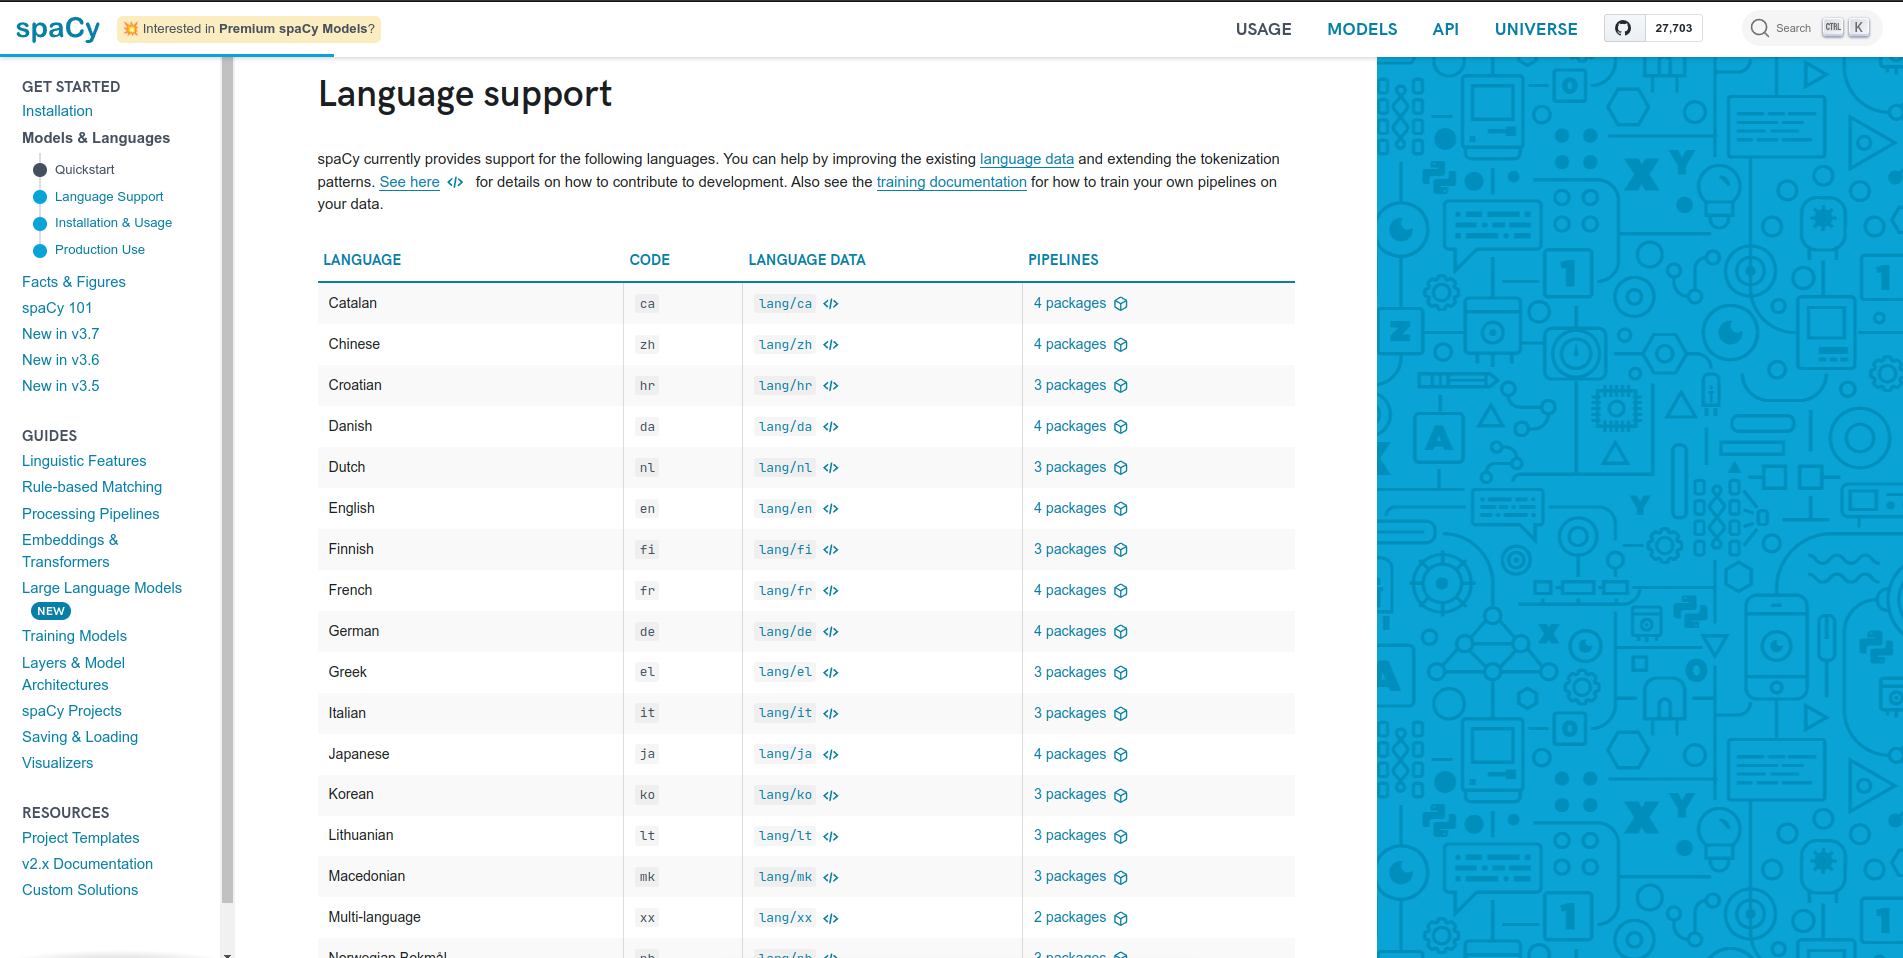
\includegraphics[width=\linewidth]{Images/SpaCy_English_Model.png}
    \caption{مدل های دارای چندین پکیج (فضای برداری کلمات از پیش آموزش دیده) در SpaCy}
\end{figure}

\begin{figure}
    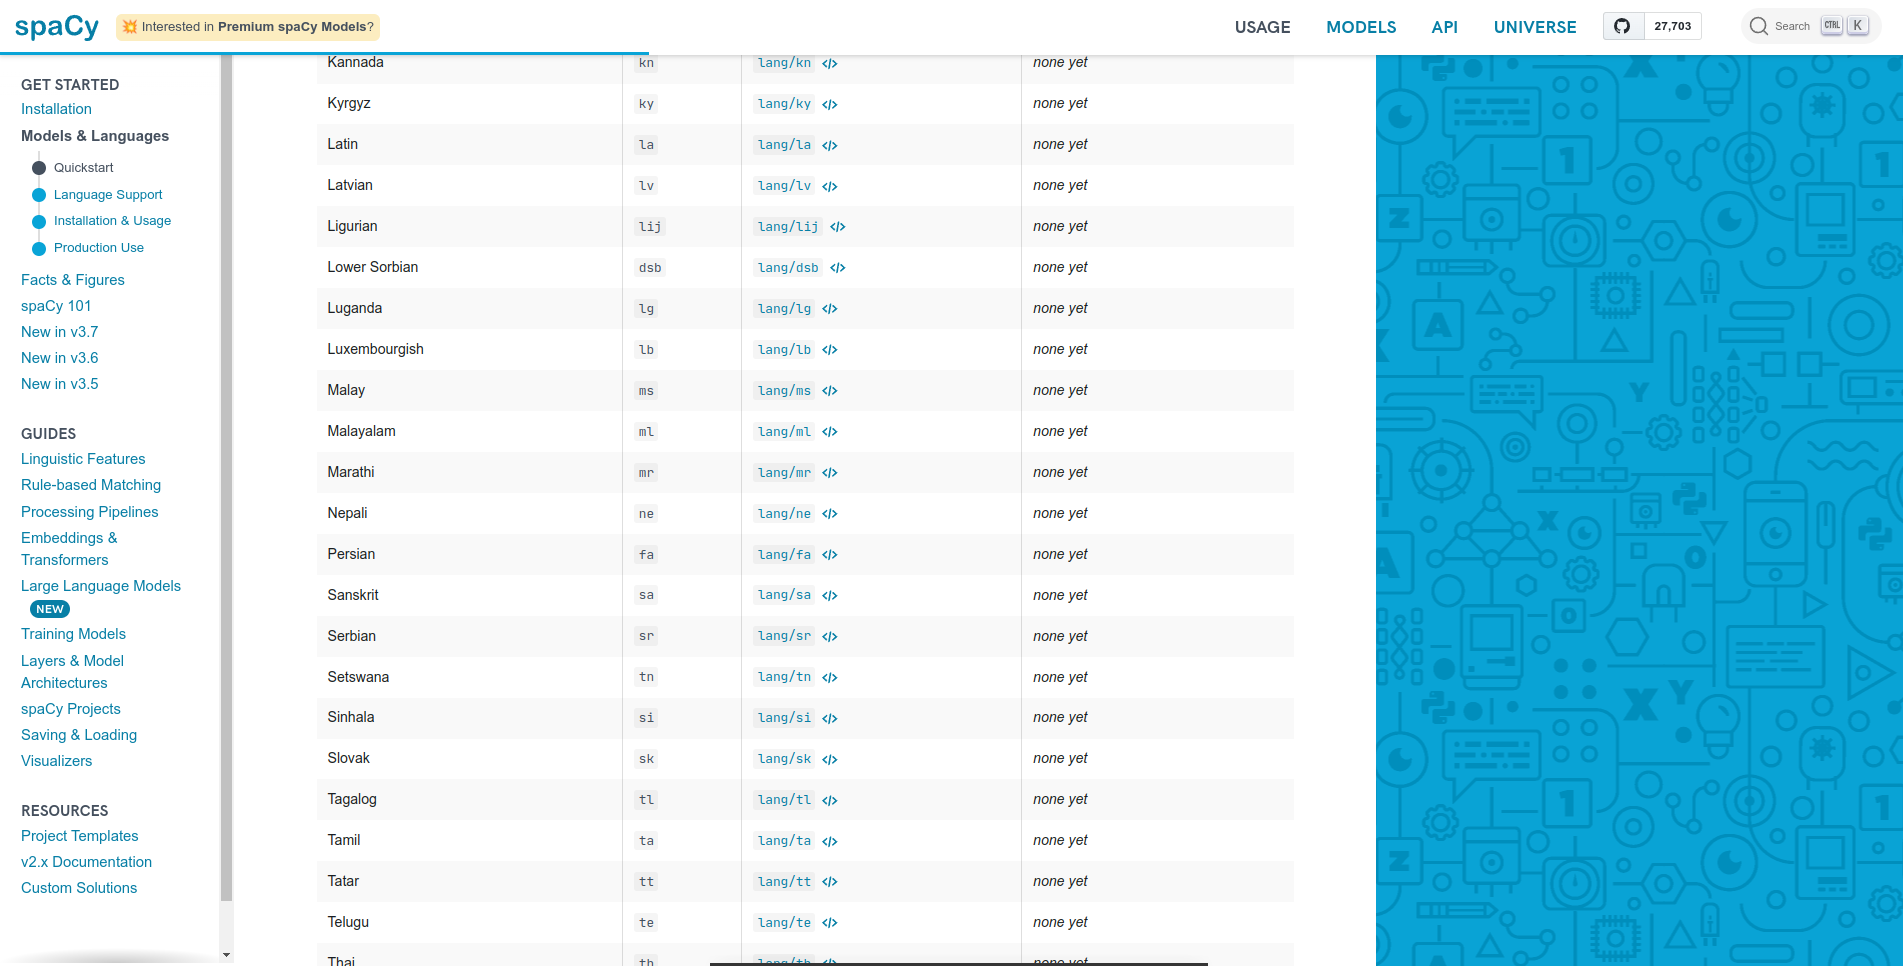
\includegraphics[width=\linewidth]{Images/SpaCy_Persian_Model.png}
    \caption{مدل زبان فارسی در SpaCy}
\end{figure}


\subsection{گزارش روز دوشنبه سیزدهم آذر‌ماه ۱۴۰۲}

۱۴۰۲/۰۹/۱۳

امروز هفته دوم دوره \lr{NLP Specialization} به جز نوت های (همان اسلایدها) این هفته و آزمون آن به اتمام رسید.


\subsection{گزارش روز سه‌شنبه چهاردهم آذر‌ماه ۱۴۰۲}

۱۴۰۲/۰۹/۱۴

در ادامه Tokenizer ها JiebaTokenizer فقط برای زبان چینی ساخته شده است 
امروز بالاخره راه درست کردن \lr{Custom Tokenizer} را پیدا کردم و بعد از اجرای دستور \lr{rasa train} متوجه شدم که علاوه بر نوع آدرس دهی که مشکل درست اجرا نشدن \lr{rasa train} بود خود کد \lr{hazm Tokenizer} ارور میدهد و بعد از کمی تحقیق متوجه شدم که همانند دیگر Tokenizer ها که در Rasa استفاده می‌شوند که در بالا یکی از آن ها مانند JiebaTokenizer  ذکر شد نیاز است برای hazm نیز از Template خاصی برای کد پایتون آن استفاده کنیم و در اولین تغییر این فایل Template برای شخصی سازی اش برای \lr{hazm Tokenizer} نیاز است که 
در @DefaultV1Recipe.register 
در قسمت ComponentType نوع کامپوننت را از نوع MESSAGE\_TOKENIZER قرار بدهیم همانند دیگر Tokenizer هایی که ذکر شد (آن ها هم نوع کامپوننت را از این نوع در نظر گرفته بودند)
بعد از این قسمت به صورت موردی پیاده سازی هر کدام از توابع در صفحه ای از \lr{Rasa Documentation} توضیح داده شده که طبق آن پیش خواهم رفت.

از دوره \lr{NLP Specialization} نیمی از اسلاید های هفته دوم را مرور کردم.



\subsection{گزارش روز چهارشنبه پانزدهم آذر‌ماه ۱۴۰۲}

۱۴۰۲/۰۹/۱۵

شبیه ترین Tokenizer ای که بین Tokenizer های نامبرده به Template موجود وجود دارد JiebaTokenizer هست و الگو گیری کلی پیاده سازی \lr{hazm Tokenizer} را از این Tokenizer انجام می‌دهم 
برای ذخیره سازی مدل که ممکن است نیاز شود به طور مثال ذخیره وزن های مدل به صورت ذخیره طولانی مدت در هارد درایو نه در RAM مدلی که Rasa برای این کار دارد \lr{Model Storage} نام دارد
چرا از روش \lr{Fast text featurizer} نمی روم و فعلا آن را کنار گذاشتم ؟ چون من آن روش را در یک issue ی قدیمی گیت هاب پیدا کردم که زمان طرح آن برای حدود 2018 بود که یعنی دو سال بعد از ساخت Rasa و یعنی حدودا برای Rasa ی دو و یا حتی یک بوده البته با اینکه این روش هنوز هم کاربرد دارد ولی چون روش قدیمی ای هست به احتمال زیاد اگر روش های جدید کاری از پیش نبردند به این روش رجوع خواهم کرد و یا حتی ممکن است برای ارتقای روش جدید از آن استفاده کنم
امروز از مرحله اجرای \lr{hazm Tokenizer} با موفقیت عبور کردم ارور بعدی برای دستور \lr{rasa train} این هست که SpaCy را نمی شناسد که در ادامه باید به آن بپردازم.


\subsection{گزارش روز پنجشنبه شانزدهم آذر‌ماه ۱۴۰۲}

۱۴۰۲/۰۹/۱۶

امروز بعد از درست کردن ارور مربوط به \lr{SpaCy Featurizer} متوجه شدم که یک Tokenizer بیشتر قابل استفاده در \lr{Rasa Pipeline} نیست و چون برای SpaCyFeaturizer نیاز بود که ابتدا یک مدل SpaCyNLP و سپس از یک SpaCyTokenizer استفاده کنیم مجبور به حذف موقت \lr{hazm Tokenizer} از پایپلاین شدم تا ببینم که آیا خود SpaCy با این که مدلی برای زبان فارسی برای آن وجود ندارد با مدل چند زبانه آن که زبان فارسی یکی از آن چند زبان هست ولی ۴ مگابایت بیشتر حجم ندارد آیا می‌توان نتیجه قابل قبولی گرفت یا خیر
بعد از با موفقیت آموزش مجدد چت بات با پایپلاین جدید (پایپلاین ای که از مدل چند زبانی SpaCy استفاده می‌کرد) اجرای مجدد چت بات هیچ پیشرفتی دیده نشد باید کمی فایل domain چت بات را عوض کنم تا ببینم آیا پیشرفتی حاصل می‌شود و یا خیر.

از دوره \lr{NLP Specialization} مرور اسلاید های هفته دوم به اتمام رسید و آزمون هفته دوم نیز گذرانده شد با دفعه سوم ۱۰۰ گرفتن.

https://github.com/JavidChaji/DeepLearning.AI-Natural-Language-Processing-Specialization


\subsection{گزارش روز جمعه هفدهم آذر‌ماه ۱۴۰۲}

۱۴۰۲/۰۹/۱۷

امروز به اصلاح فایل های Rasa پرداختم و در نهایت تا حدودی توانستم نتیجه بهتری از دیروز در مکالمه با چت بات بگیرم ولی یک مشکل دیگر که امروز درگیر آن بودم این بود که وقتی که کاربر از چت ویجت استفاده می‌کند برای پیام دادن به Agent که یعنی من و یا چت بات این پیام را چطوری به دست چت بات برسانم و بعد از حل این مشکل سوال بزرگتر این که اگر چندین کاربر همزمان بخواهند از Rasa سوال بپرسند چطور!!!
و همینطور کمی با توجه به نتایج گرفته شده از گفتگو با چت بات به برداشتم از مفهوم مدل زبانی ای که به Pipeline اضافه کردم شک کردم که فردا باید بررسی کنم .

از دوره \lr{NLP Specialization} قسمت مقدمه هفته سوم و \lr{N-grams Overview} را گذراندم .

https://github.com/JavidChaji/DeepLearning.AI-Natural-Language-Processing-Specialization


\subsection{گزارش روز شنبه هجدهم آذر‌ماه ۱۴۰۲}

۱۴۰۲/۰۹/۱۸

امروز شکی که به برداشت اشتباه از مدل برایم پیش آمده بود را چک کردم و مشکلی وجود نداشت، اما مهمترین قسمت از اینجا به بعد فقط و فقط و فقط خیلی به داده وابسته هست
همین طور که به یافتن داده مناسب فکر می‌کردم درباره داده های موجود فارسی جستجو کردم و به ParsBERT رسیدم که یک مدل بسیار خوب برای زبان فارسی است این مدل در \lr{Hugging Face} موجود هست ولی برای اضافه کردن آن به پایپلاین Rasa راه ساده ای پیدا نکردم مجدداً فردا به دنبال راهی برای اضافه کردن این مدل به Rasa میگردم به نظر می‌آید افراد دیگر هم که قبلاً تلاش برای اضافه کردن مدل های \lr{Hugging Face} به Rasa نتیجه ای نگرفته اند و بعضاً Froum هایی که از آن ها به این نتیجه رسیدم Froum های قدیمی ای هستند که احتمالاً برای Rasa نسخه ۱ مطرح شدند ولی البته راجع به اضافه کردن LLM ها به Rasa در Documentation آن چیزی نوشته نشده است ولی Rasa چیزی تحت عنوان \lr{Beta Documentation} دارد که در آن مواردی که در آینده به زودی قرار است به Rasa اضافه شوند را مستند می کند و توضیح ناقص و کمی از اضافه کردن مدل های \lr{Hugging Face} به خود را نیز می‌دهد.

از دوره \lr{NLP Specialization} قسمت مربوط به \lr{N-grams and Probabilities} را گذراندم.

https://github.com/JavidChaji/DeepLearning.AI-Natural-Language-Processing-Specialization


\subsection{گزارش روز یکشنبه نوزدهم آذرماه ۱۴۰۲}

۱۴۰۲/۰۹/۱۹

امروز برای سریع تر پیش رفتن پروژه و رسیدن به کارهای عملی ای که پروژه را تکمیل می‌کند به دنبال یک مثال خوب از یک چت بات آموزشی بودم (از بین چت بات هایی که با Rasa نوشته شده بودند.) که با الگو گیری از Intent ها و پاسخ های آن چت بات را تکمیل کنم ولی مثال خوبی در این زمینه وجود نداشت اما مثال هایی وجود داشتند که بشود از آن ها کمک گرفت مثل Sara که یک نمونه چت بات کامل هست که توسط خود سازندگان Rasa نوشته شده تا با تعامل با آن اگر درباره Rasa سوالی داشته باشید بپرسید کد آن هم در گیت هاب خود Rasa یعنی RasaHQ موجود هست. این از مثال نه چندان شبیه؛ قسمت بعدی پیداکردن یک منبع قانون خوب برای پاسخ به سوالات آموزشی دانشجویان دانشگاه فردوسی مشهد بود یک شیوه نامه\cite{1} از سایت آموزش کل پیدا کردم که آخرین ویرایش هم هست و مربوط به قوانین آموزشی است که به احتمال زیاد این آیین نامه را در قالب پرسش و پاسخ (با طرح پرسش و پاسخ و قرار دادن آن ها در فایل های داده های \lr{train}) در اختیار Rasa خواهم گذاشت تا به عنوان داده برای چت بات استفاده شود.

از دوره \lr{NLP Specialization} قسمت مربوط به \lr{Sequence Probabilities} را گذراندم.

https://github.com/JavidChaji/DeepLearning.AI-Natural-Language-Processing-Specialization


\subsection{گزارش روز دوشنبه بیستم آذر‌ماه ۱۴۰۲}

۱۴۰۲/۰۹/۲۰

امروز از شیوه نامه آموزشی سوال هایی به عنوان Intent طرح کردم که چند تا از تعاریف شیوه نامه را به عنوان پاسخ نیاز داشت، این سوال ها به فایل nlu.yml اضافه کردم و برای هر کدام حدود ۱۵ سوال طرح کردم تا به عنوان داده برای Train چت بات استفاده شود و پاسخ ها هم در قسمت Response در فایل domain.yml قرار گرفت. (دقیقا بر طبق شیوه نامه)

از دوره NLP Specialization قسمت \lr{Starting and Ending Sentences} را گذراندم یا مدرس خیلی مبهم تدریس کرد و یا برای من کمی هضم اینکه چرا انتهای هر جمله در \lr{N-gram model} رشته ی <\textbackslash s> را فقط یک بار اضافه میکنیم نه N-1 بار، مانند رشته <s> در ابتدای جمله ها ولی احتمالا در جلسات آینده توضیح دقیق تری خواهد داد در غیر این صورت با نوشتن یک مثال و تست کردن این مورد که چرا باید مجموع احتمالات N-gram های یک Corpus یک شود سعی می‌کنم تا دلیل آن را بیابم.

https://github.com/JavidChaji/DeepLearning.AI-Natural-Language-Processing-Specialization


\subsection{گزارش روز سه‌شنبه بیست و یکم آذر‌ماه ۱۴۰۲}

۱۴۰۲/۰۹/۲۱

امروز در ادامه تبدیل شیوه‌نامه به داده قابل آموزش تا تعریف دهم از تعاریف شیوه‌نامه پیش رفتم و برای گرفتن تست از اینکه چت بات تا اینجا درست کار می کند یا خیر سعی کردم یک Story برای پرسیدن این سوال ها بنویسم برای همین شروع به کردم به چک کردن Story های مختلف مربوط به Sara  از چند عدد از Story های Sara الگو گرفتم ولی هنوز به خوبی Story های مرتبط تر را چک نکرده ام تا یک Story مناسب برای سوالات طراحی شده پیدا کنم کمی باید طرح اصولی تر Story را مجدداً چک کنم (در حد نیم ساعت).

از دوره \lr{NLP Specialization} قسمت \lr{The N-gram Language Model} را گذراندم. خیلی جالبه الان متوجه میشم N-gram هایی که در \lr{Hugging Face} در قسمت \lr{Llama 2} گفته شده بود منظورشون چیزی شبیه به این ها بوده است.

https://github.com/JavidChaji/DeepLearning.AI-Natural-Language-Processing-Specialization


\subsection{گزارش روز چهارشنبه بیست و دوم آذر‌ماه ۱۴۰۲}

۱۴۰۲/۰۹/۲۲

امروز Story های چت بات مثال (Sara) را بیشتر بررسی کردم و در مورد اینکه چگونه می‌شود که یک سناریو ی خوب برای پرسش از شیوه نامه نوشت پیدا نکردم فردا مجدداً با آزمون و خطا اینکه چه سناریو ای بهتر خواهد بود برای این موضوع را چک می‌کنم.


\subsection{گزارش روز پنجشنبه بیست و سوم آذر‌ماه ۱۴۰۲}

۱۴۰۲/۰۹/۲۳

امروز از نوشتن چند Story شروع کردم و در نهایت متوجه شدم اشکالاتی در نحوه نوشتن Intent ها و Action ها دارم مثل این که برای بعضی از Intent ها utter در ابتدای نام آن ها گذاشته بودم در حالی که این پیشوند را فقط برای action ها به کار می‌برند و بعضاً هم بلعکس جایی که utter نیاز داشت ننوشته بودم که تا حد زیادی اصلاح شد و کمی ارور دیگر دارد که در زمان اجرای دستور \lr{rasa train} نمایش داده می‌شود که اکثراً مربوط به همین اشکال ذکر شده اند که با رفع آن ها فردا چت بات را با داده های کم فعلی تست خواهم کرد.


\subsection{گزارش روز جمعه بیست و چهارم آذر‌ماه ۱۴۰۲}

۱۴۰۲/۰۹/۲۴

امروز رفع اشکالات موجود در داده های آموزشی انجام شد و چت بات مورد تست قرار گرفت. جالب بود و پاسخ های نسبتاً خوبی به سوالات می‌داد و تقریباً به جز یک مورد که کمی خطا بود و موردی دیگر که اشکال مدل آموزشی خودم بود خطای خاصی نداشت و به خوبی \lr{Intent Classification} برای زبان فارسی انجام می‌گرفت حس جالبی بود که مثلاً یکی از گزینه های جواب برای خداحافظی اش را به شوخی بای بای قرار داده بودم که به احتمال یک ششم پاسخش به خداحافظی خواهد بود (چون از هر پاسخی که در اختیارش در داده های آموزشی میگذاریم احتمال انتخاب شدن آن پاسخ با بقیه مساوی است) و یک دفعه که از چت بات پرسیدم تعریف یک اصطلاح چیست بعد از توضیح آن با توجه به کشف Intent من به آن پاسخ داد و سپس گفت آیا پاسخ خود را گرفتید و بعد از گفتن بله، گفت بای بای انگار که سریع پاسخ من را داد که از دست من راحت شود.

از دوره \lr{NLP Specialization} قسمت Evaluation که بیشتر معرفی Perplexity بود را مشاهده کردم.

https://github.com/JavidChaji/DeepLearning.AI-Natural-Language-Processing-Specialization


\subsection{گزارش روز شنبه بیست و پنجم آذر‌ماه ۱۴۰۲}

۱۴۰۲/۰۹/۲۵

امروز بالاخره موفق شدم ارتباط \lr{Chat Widget} با Rasa را برقرار کنم الان اگر در گوشه پایین سمت راست سایت \lr{Chat Widget} را باز کرده و از او سوالی بپرسید Rasa پاسخ شما را خواهد داد البته نه خیلی مناسب و همینجاست که چون این تست ها و آزمایشات روی Rasa و Rocket.Chat نتیجه داده باید به مرتب کردن کامل داده های آموزشی و اضافه کردن داده های باقی مانده (تقریبا ۹۶ درصد داده ها)
از شیوه نامه آموزشی بپردازم.

از دوره \lr{NLP Specialization} قسمت \lr{out of vocabulary words}  را گذراندم که درباره روش های مدیریت کلماتی که در فرهنگ لغت ما وجود ندارد بحث شد.

https://github.com/JavidChaji/DeepLearning.AI-Natural-Language-Processing-Specialization


\subsection{گزارش روز یکشنبه بیست و ششم آذر‌ماه ۱۴۰۲}

۱۴۰۲/۰۹/۲۶

امروز قسمت تعاریف شیوه نامه به عنوان پاسخ به چت بات اضافه شد ولی هنوز برای همه آن ها Intent تعریف نشده است قبل از تعریف Intent برای آن ها سعی می‌کنم که به ماده ها و تبصره های شیوه نامه بپردازم و تا جایی که زمان اجازه دهد آن ها را هم به پاسخ های چت بات اضافه کنم و سپس به اضافه کردن Intent به ادامه تعاریف و همچنین ماده ها و تبصره ها خواهم پرداخت.

از دوره \lr{NLP Specialization} قسمت Smoothing را مشاهده کردم که درباره روش های رفتار با N-gram های بدون احتمال و یا با احتمال صفر بود که روش های Smoothing, Backoff, Interpolation معرفی شد برای مدیریت این N-gram ها.

https://github.com/JavidChaji/DeepLearning.AI-Natural-Language-Processing-Specialization


\subsection{گزارش روز دوشنبه بیست و هفتم آذر‌ماه ۱۴۰۲}

۱۴۰۲/۰۹/۲۷

امروز در ادامه تبدیل شیوه نامه به داده های قابل آموزش برای Rasa شروع به اضافه کردن ماده ها و تبصره های مربوط به تمام سطوح تحصیلی یعنی فصل اول شیوه‌نامه کردم و در پایان اضافه کردن این Response ها باید Intent مربوط به هر یک را با مثال های مناسب در فایل nlu.yml بنویسم.

از دوره \lr{NLP Specialization} قسمت \lr{Week Summery} را مشاهده کردم.

https://github.com/JavidChaji/DeepLearning.AI-Natural-Language-Processing-Specialization


\subsection{گزارش روز سه‌شنبه بیست و هشتم آذر‌ماه ۱۴۰۲}

۱۴۰۲/۰۹/۲۸

امروز قسمت Respone ها را برای فصل اول شیوه نامه کامل کردم و قسمت بعدی  برای فردا شروع به اضافه کردن Intent این Response ها به فایل nlu.yml است.


\subsection{گزارش روز چهارشنبه بیست و نهم آذر‌ماه ۱۴۰۲}

۱۴۰۲/۰۹/۲۹

امروز شروع به نوشتن Intent های متناسب با ماده ها و تبصره های شیوه نامه کردم و تعریف تمامی Intent ها را در فایل domain.yml اضافه کردم و همینطور Intent های تعاریف باقی مانده را اضافه کردم و الان فقط باید شروع به نوشتن مثال های مختلف به ازای هر Intent کنم مانند پرسش های مختلفی که قصد آن ها رسیدن به همان ماده و یا تبصره ای باشد که برایش مثال می‌نویسیم.

\subsection{گزارش های بعد از بیست و نهم آذرماه}

بعد از این تاریخ مشغول ساخت و آماده‌سازی این مستندات برای ارائه بودم.




\newpage
    

\end{document}
